\documentclass[aspectratio=169]{beamer}

\usepackage{graphicx}
\usepackage{subcaption}
\usepackage{amsmath,amssymb,amsfonts}
\usepackage{algorithmic}
\usepackage{graphicx}
\usepackage{textcomp}
\usepackage{xcolor}
\usepackage{hyperref}
\usetheme{Boadilla}
\usepackage{cite}
\usepackage{animate}

\definecolor{mypurple}{RGB}{71, 71, 187}
\definecolor{subpurple}{RGB}{133, 133, 208}
\definecolor{subsubpurple}{RGB}{173, 173, 224}
\setbeamercolor{title}{bg=mypurple, fg=white}
% \setbeamercolor{frametitle}{bg=subsubpurple, fg=white}
% -------------------------------------------------------------
% Title Page
% -------------------------------------------------------------
\title{\textbf{Multi-UAV Source Seeking and Optimization}}
\subtitle{\textit{BTP Project}}
\author{
    \textit{Dikshant (2022102038) }, \\
    \textit{Dr. Harikumar Kandath}
}
\date{\texttt{\today}}

\begin{document}

\begin{frame}
\titlepage 
\end{frame}
\author{
    \textit{Dikshant }, \\
    \textit{Dr. Harikumar Kandath}
}

% % % % ------------------------ PSO ------------------------
\begin{frame}{PSO}
    PSO is the technique used to find an approximate solution for maximization or minimization problems.
    \begin{itemize}
        \item PSO is initialized with a group of random particles (solutions) and then searches for the optimal solution by updating generations.
        \item Particles move through the solution space, and are evaluated according to some fitness criterion after each time step. In every iteration, each particle is updated by following two "best values".
        \item The first one is the best solution (fitness) it has achieved so far (the fitness value is also sorted). This value is called \textbf{$P_{best}$}.
        \item Another best value that is tracked by the PSO is the best value obtained so far by any particle in the population. This second-best value is a \textbf{global best} and called \textbf{$g_{best}$}.
    \end{itemize}
\end{frame}

% % % % ------------------------ Objective ------------------------
\begin{frame}{Objective}
\textbf{Source Seeking:}
    \begin{itemize}
        \item Understand \cite{10312321} and reproduce its results.
    \end{itemize}

\textbf{Optimization:}
    \begin{itemize}
        \item Using CEC2022 benchmarks \cite{luo2022benchmarkfunctionscec2022} for optimization of \cite{10312321} PSO algorithms.
        \item To develop and evaluate hybrid Particle Swarm Optimization approaches that combine the strengths of different PSO variants
        \item To improve optimization performance on complex benchmark functions through strategic algorithm hybridization
        \item To analyze how different hybridization strategies affect convergence behavior and solution quality
        \item To identify which hybrid approaches are most effective for specific types of optimization problems
    \end{itemize}
    
\end{frame}

% % % % ------------------------ APSO ------------------------
\begin{frame}{APSO (Acceleration based PSO)}
    \begin{itemize}
        \item Uses acceleration as the primary update mechanism (second-order dynamics)
        \item Maintains momentum through previous movement history
        \item Produces smoother trajectories with more consistent direction
    \end{itemize}
    
    \textbf{Mathematical Formulation:} \\
    \begin{itemize}
        \item \textbf{acc update:} $a_i(t+1) = \omega_{1} a
    _i(t) + c_1 r_1(p_i - x_i) + c_2r_2(g-x_i)$
        \item \textbf{Velocity update:} $v_i(t+1) = \omega_2v_i(t) + a_i(t+1)T$
        \item \textbf{Position update:} $x_i(t+1) = x_i(t) + v_i(t+1)T$
    \end{itemize}
\end{frame}

% % % % ------------------------ SPSO ------------------------
\begin{frame}{SPSO (Standard PSO)}
    \begin{itemize}
        \item Direct velocity-based update mechanism (first-order dynamics)
        \item Balanced exploration-exploitation trade-off
        \item Widely used baseline algorithm in swarm intelligence
    \end{itemize}
    
    \textbf{Mathematical Formulation:} \\
    \begin{itemize}
        \item \textbf{Velocity update:} $v_i(t+1) = \omega_{1} v
    _i(t) + c_1 r_1(p_i - x_i) + c_2r_2(g-x_i)$
        \item \textbf{Position update:} $x_i(t+1) = x_i(t) + v_i(t+1)$
    \end{itemize}
\end{frame}

% % % % ------------------------ ARPSO ------------------------
\begin{frame}{ARPSO (Adaptive Random PSO)}
    \begin{itemize}
        \item Incorporates adaptive parameters and randomness
        \item Dynamically adjusts inertia weight based on swarm state
        \item Includes additional random attractive positions for exploration
    \end{itemize}
    
    \textbf{Mathematical Formulation:} \\
    \begin{itemize}
        \item \textbf{Adaptive inertia:} $\omega_i(t+1) = f(evolutionary speed, aggregation degree)$
        \item \textbf{Velocity update:} $v_i(t+1) = \omega_iv_i(t) + c_1r_1(p_i-x_i) + c_2r_2(g-x_i) + c_3r_3(a_i-x_i)$
        \item here $a_i$ is a random attractive position
        \item \textbf{Position update:} $x_i(t+1) = x_i(t) + v_i(t+1)$
    \end{itemize}

    \textbf{NOTE:} For code all the values were taken from the paper \cite{10312321}.
\end{frame}
% % % % ------------------------ Source Seeking without noise ------------------------
\begin{frame}{Source Seeking without noise}    
    \begin{figure}[h]
        \centering
        \begin{subfigure}[b]{0.32\textwidth}
            \centering
            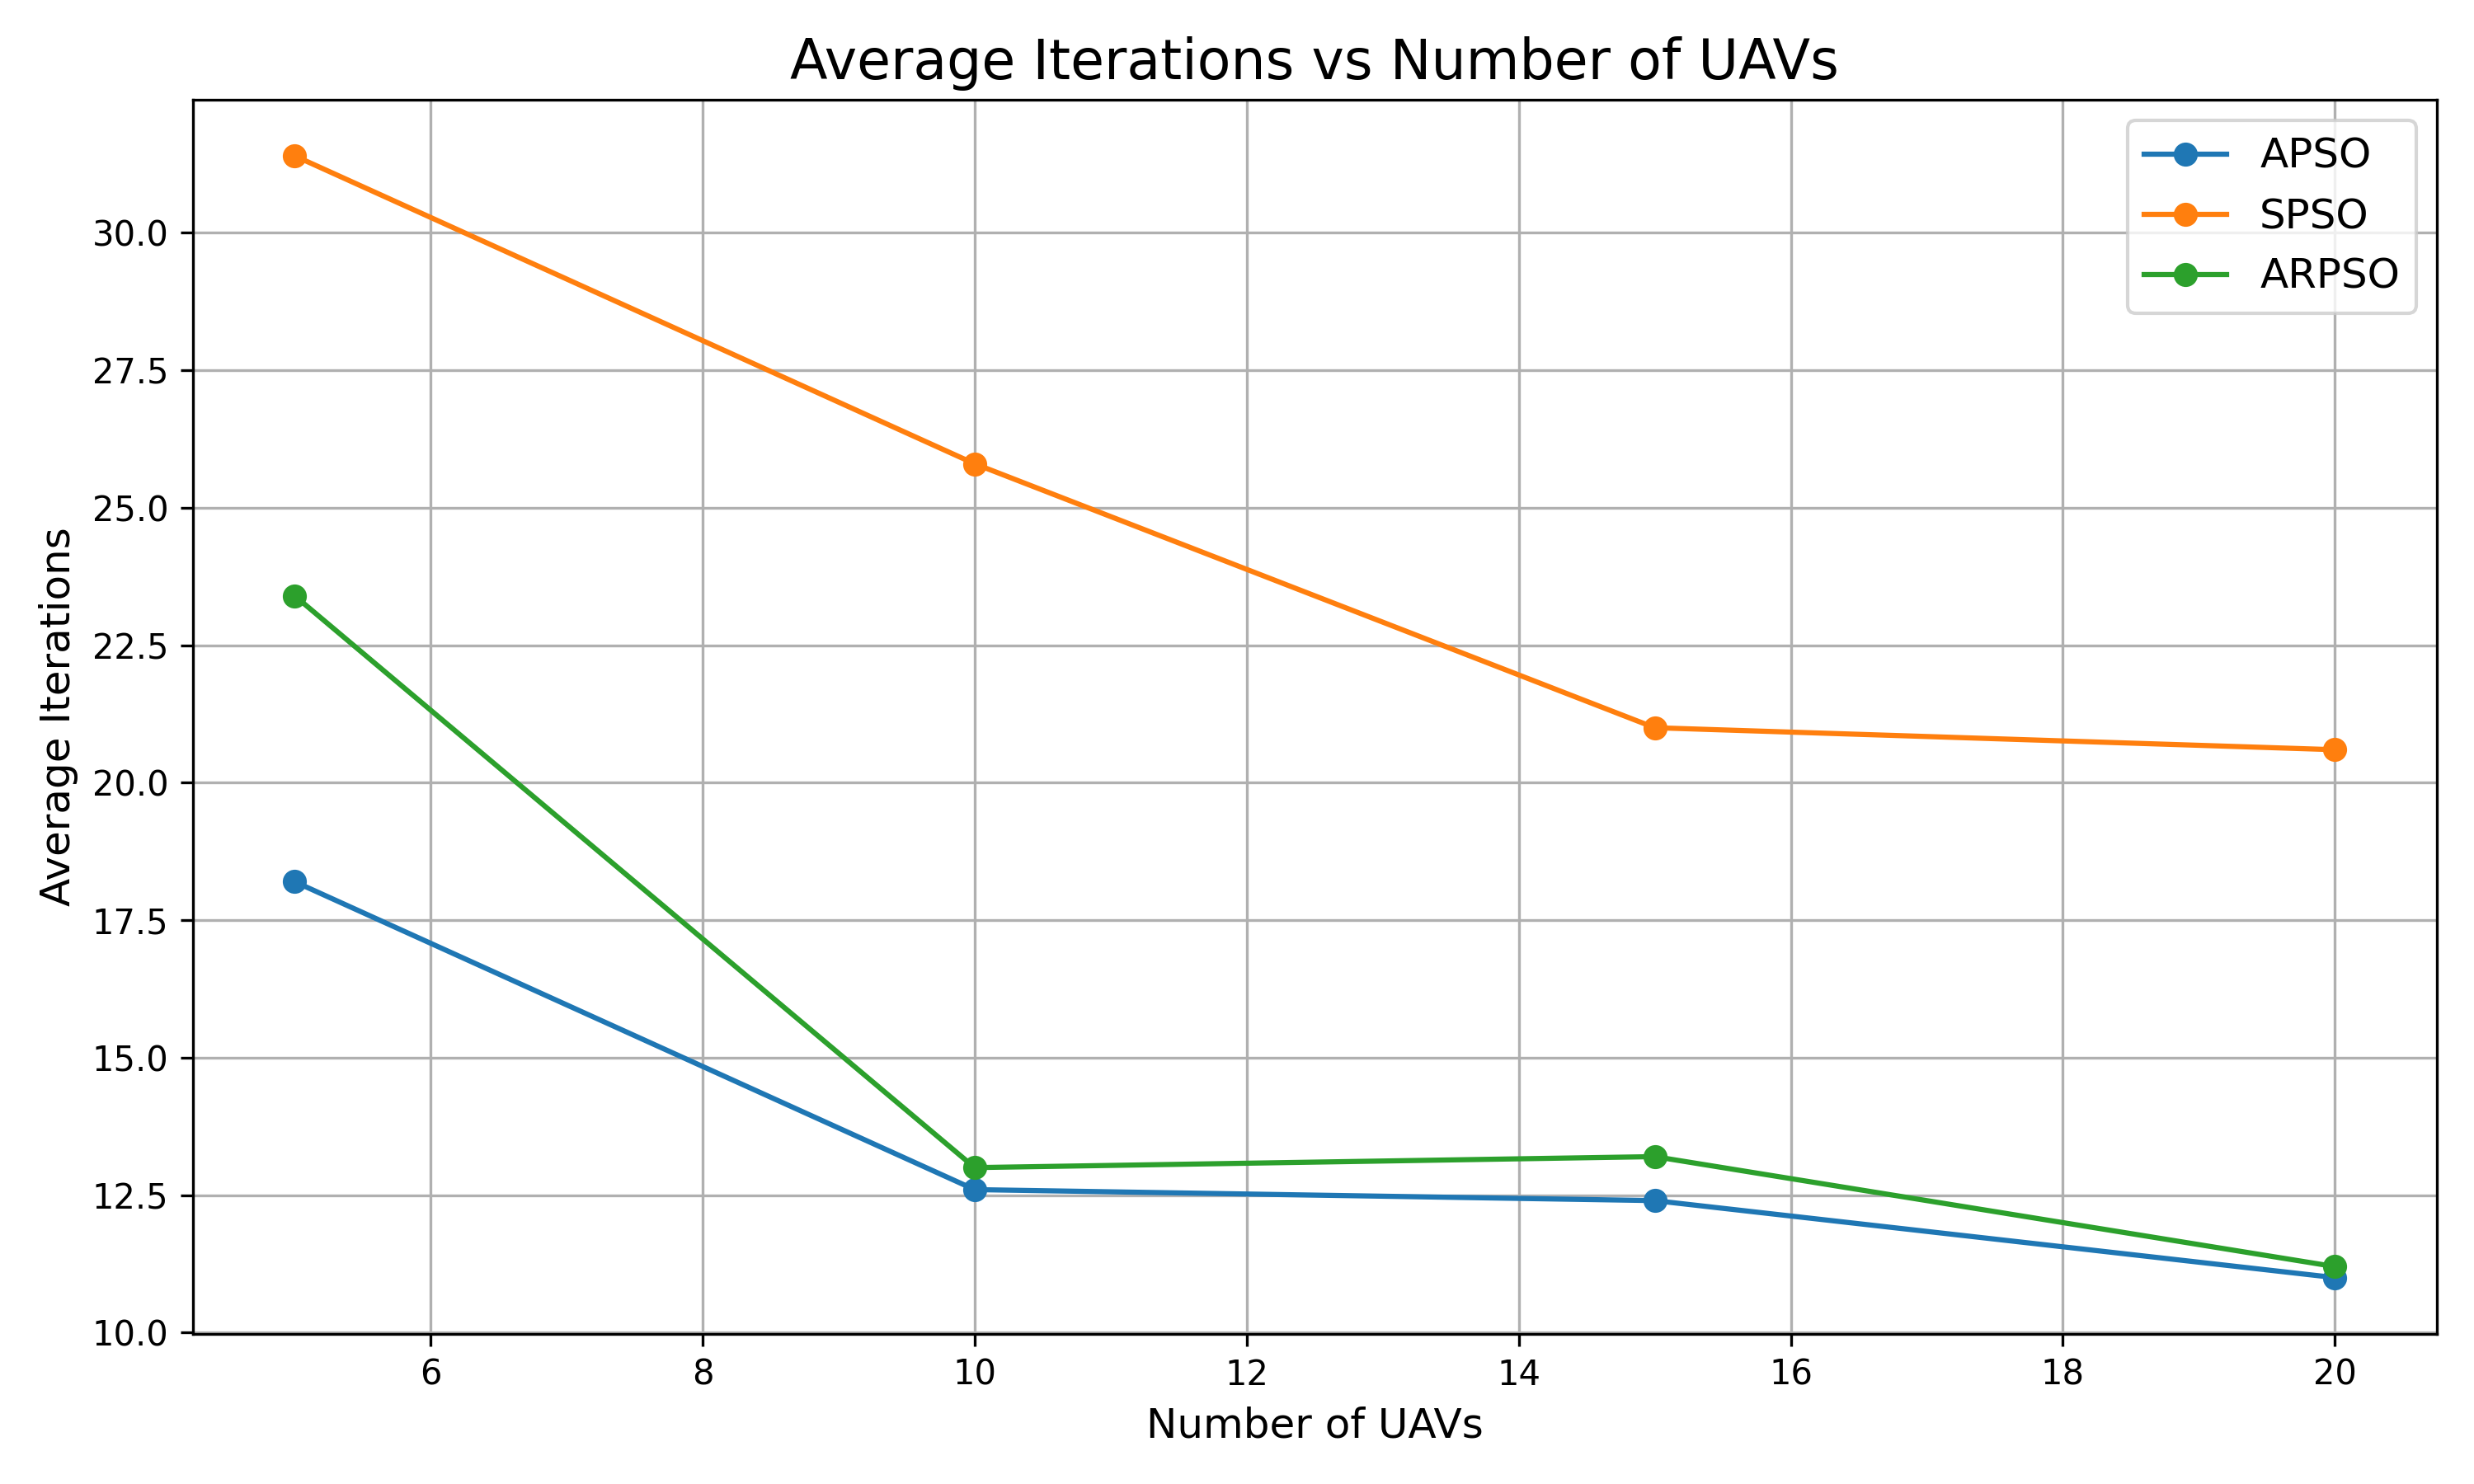
\includegraphics[width=\textwidth]{../plots/r2_without_noise/iterations_vs_#UAVs.png}
            \caption{iterations vs No. of UAV's}
        \end{subfigure}
        \hfill
        \begin{subfigure}[b]{0.32\textwidth}
            \centering
            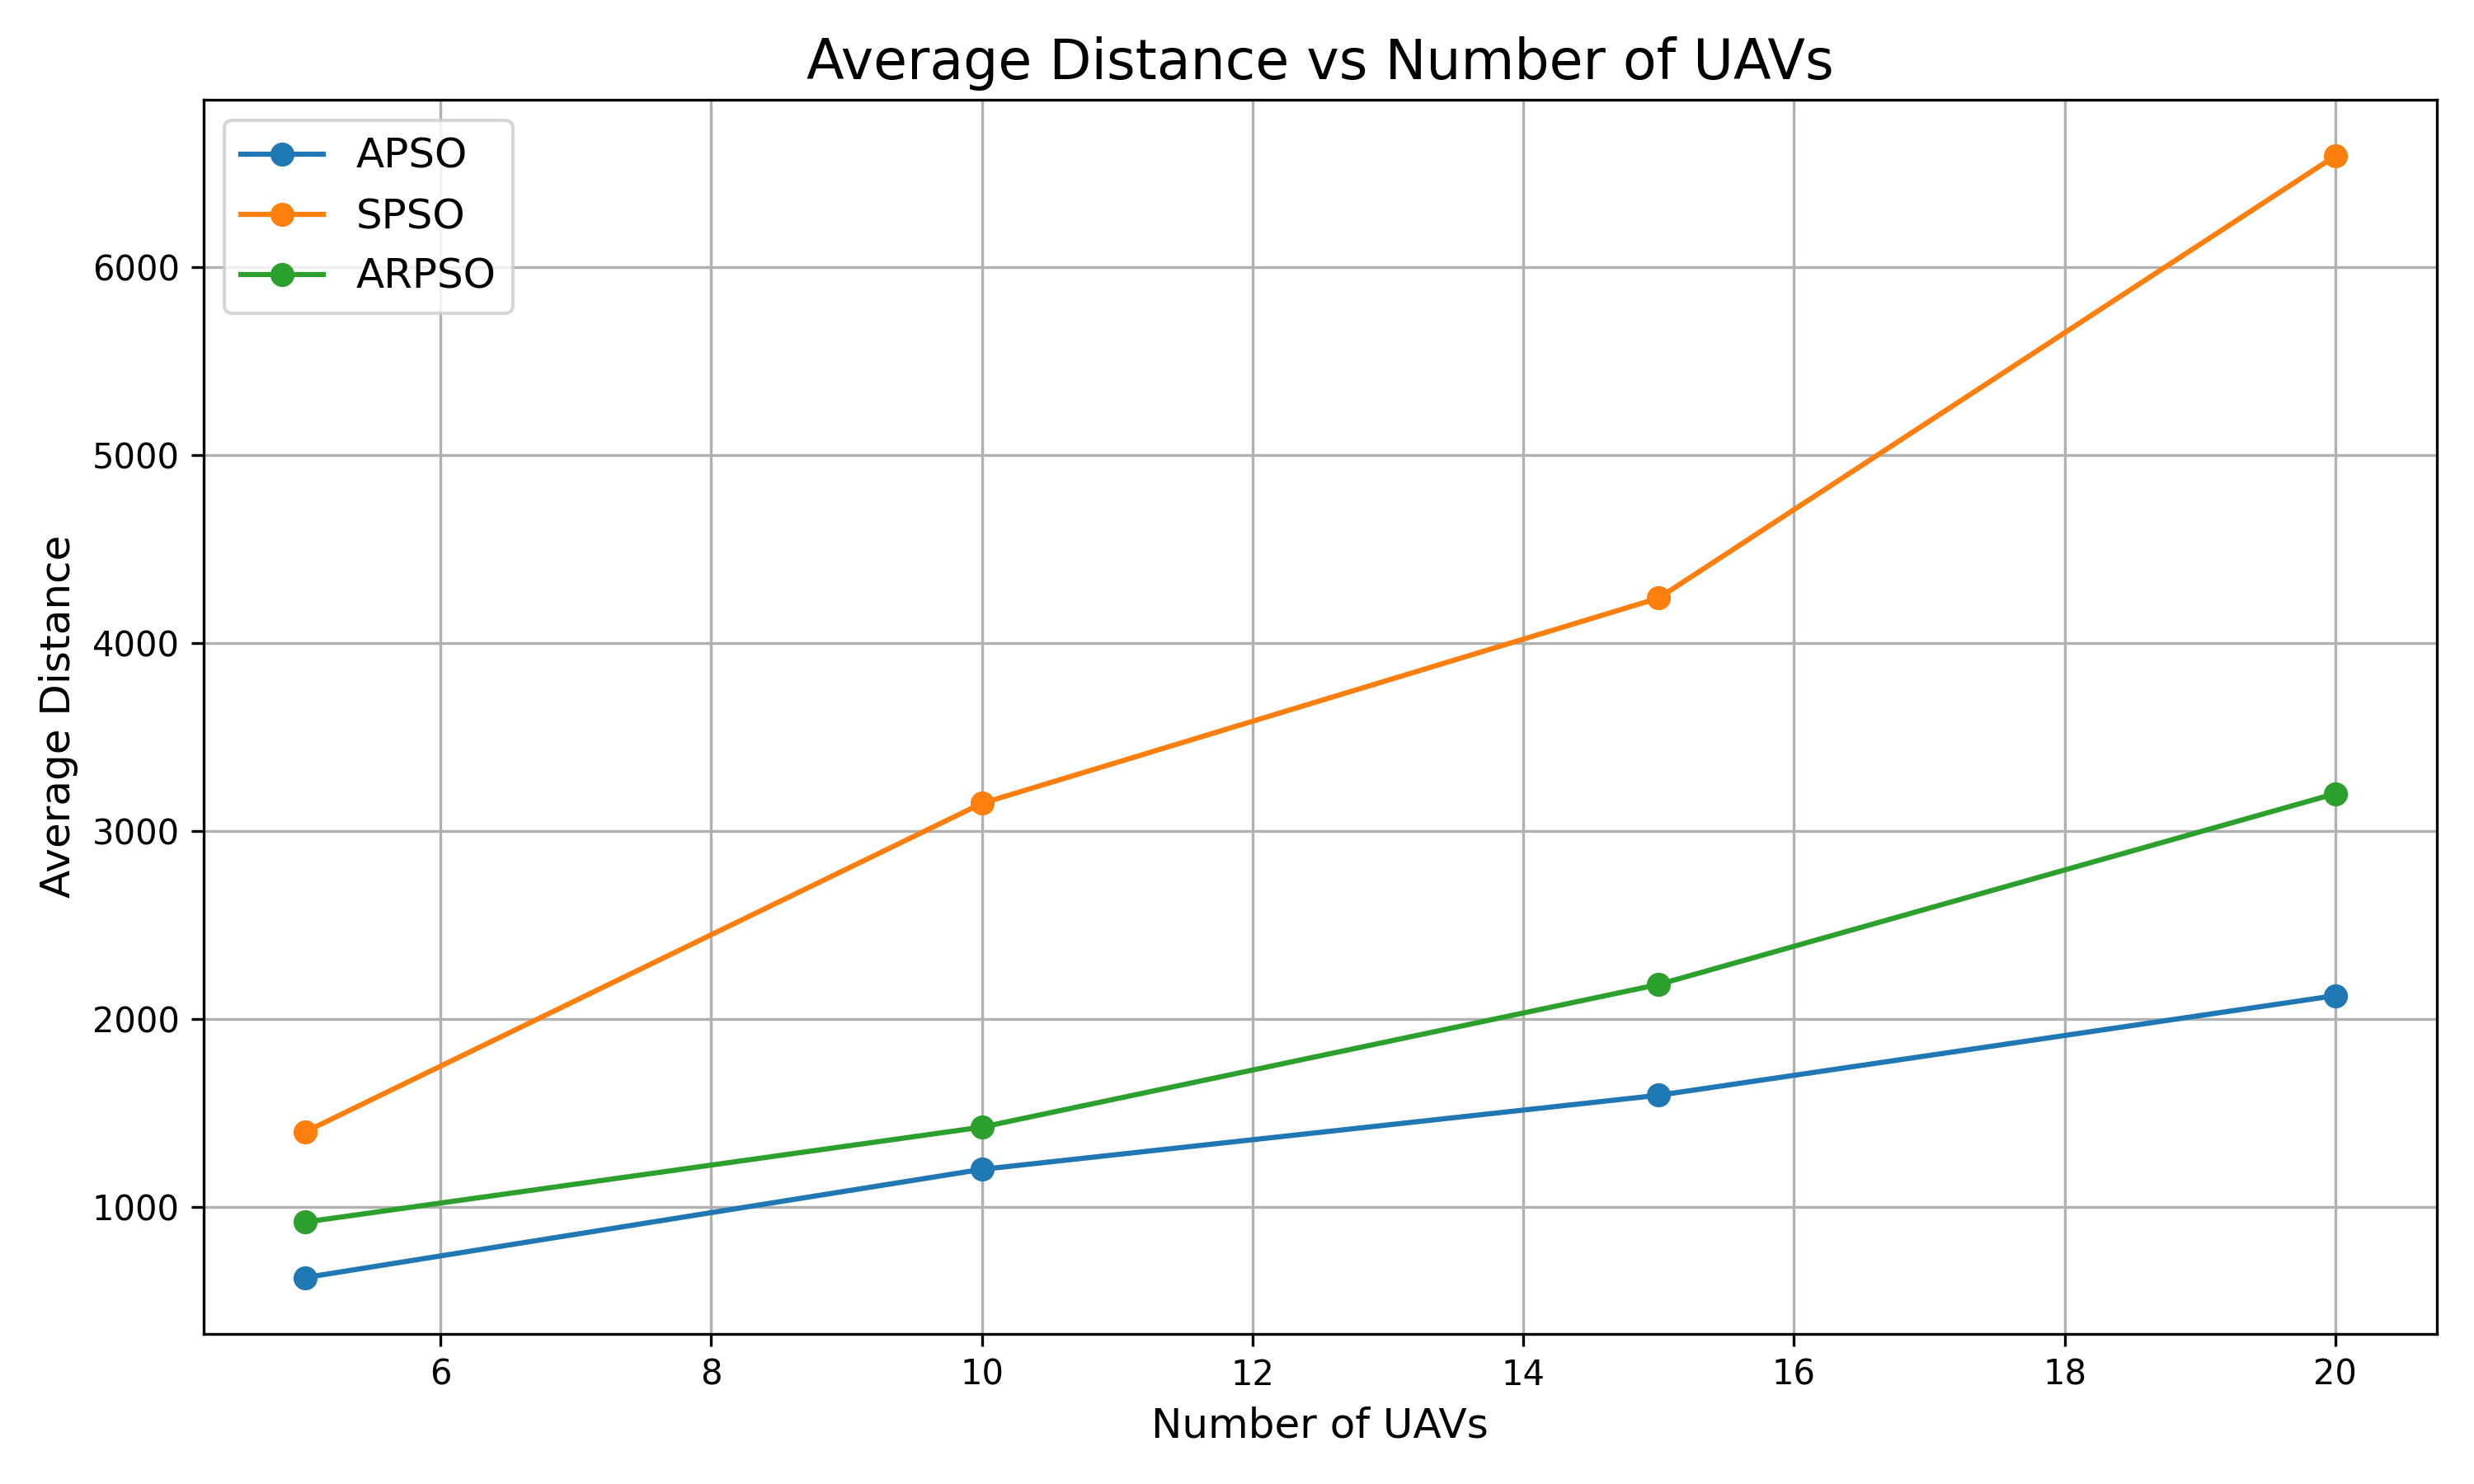
\includegraphics[width=\textwidth]{../plots/r2_without_noise/distance_vs_#UAVs.png}
            \caption{Distance vs No. of UAV's}
        \end{subfigure}
        \hfill
        \begin{subfigure}[b]{0.32\textwidth}
            \centering
            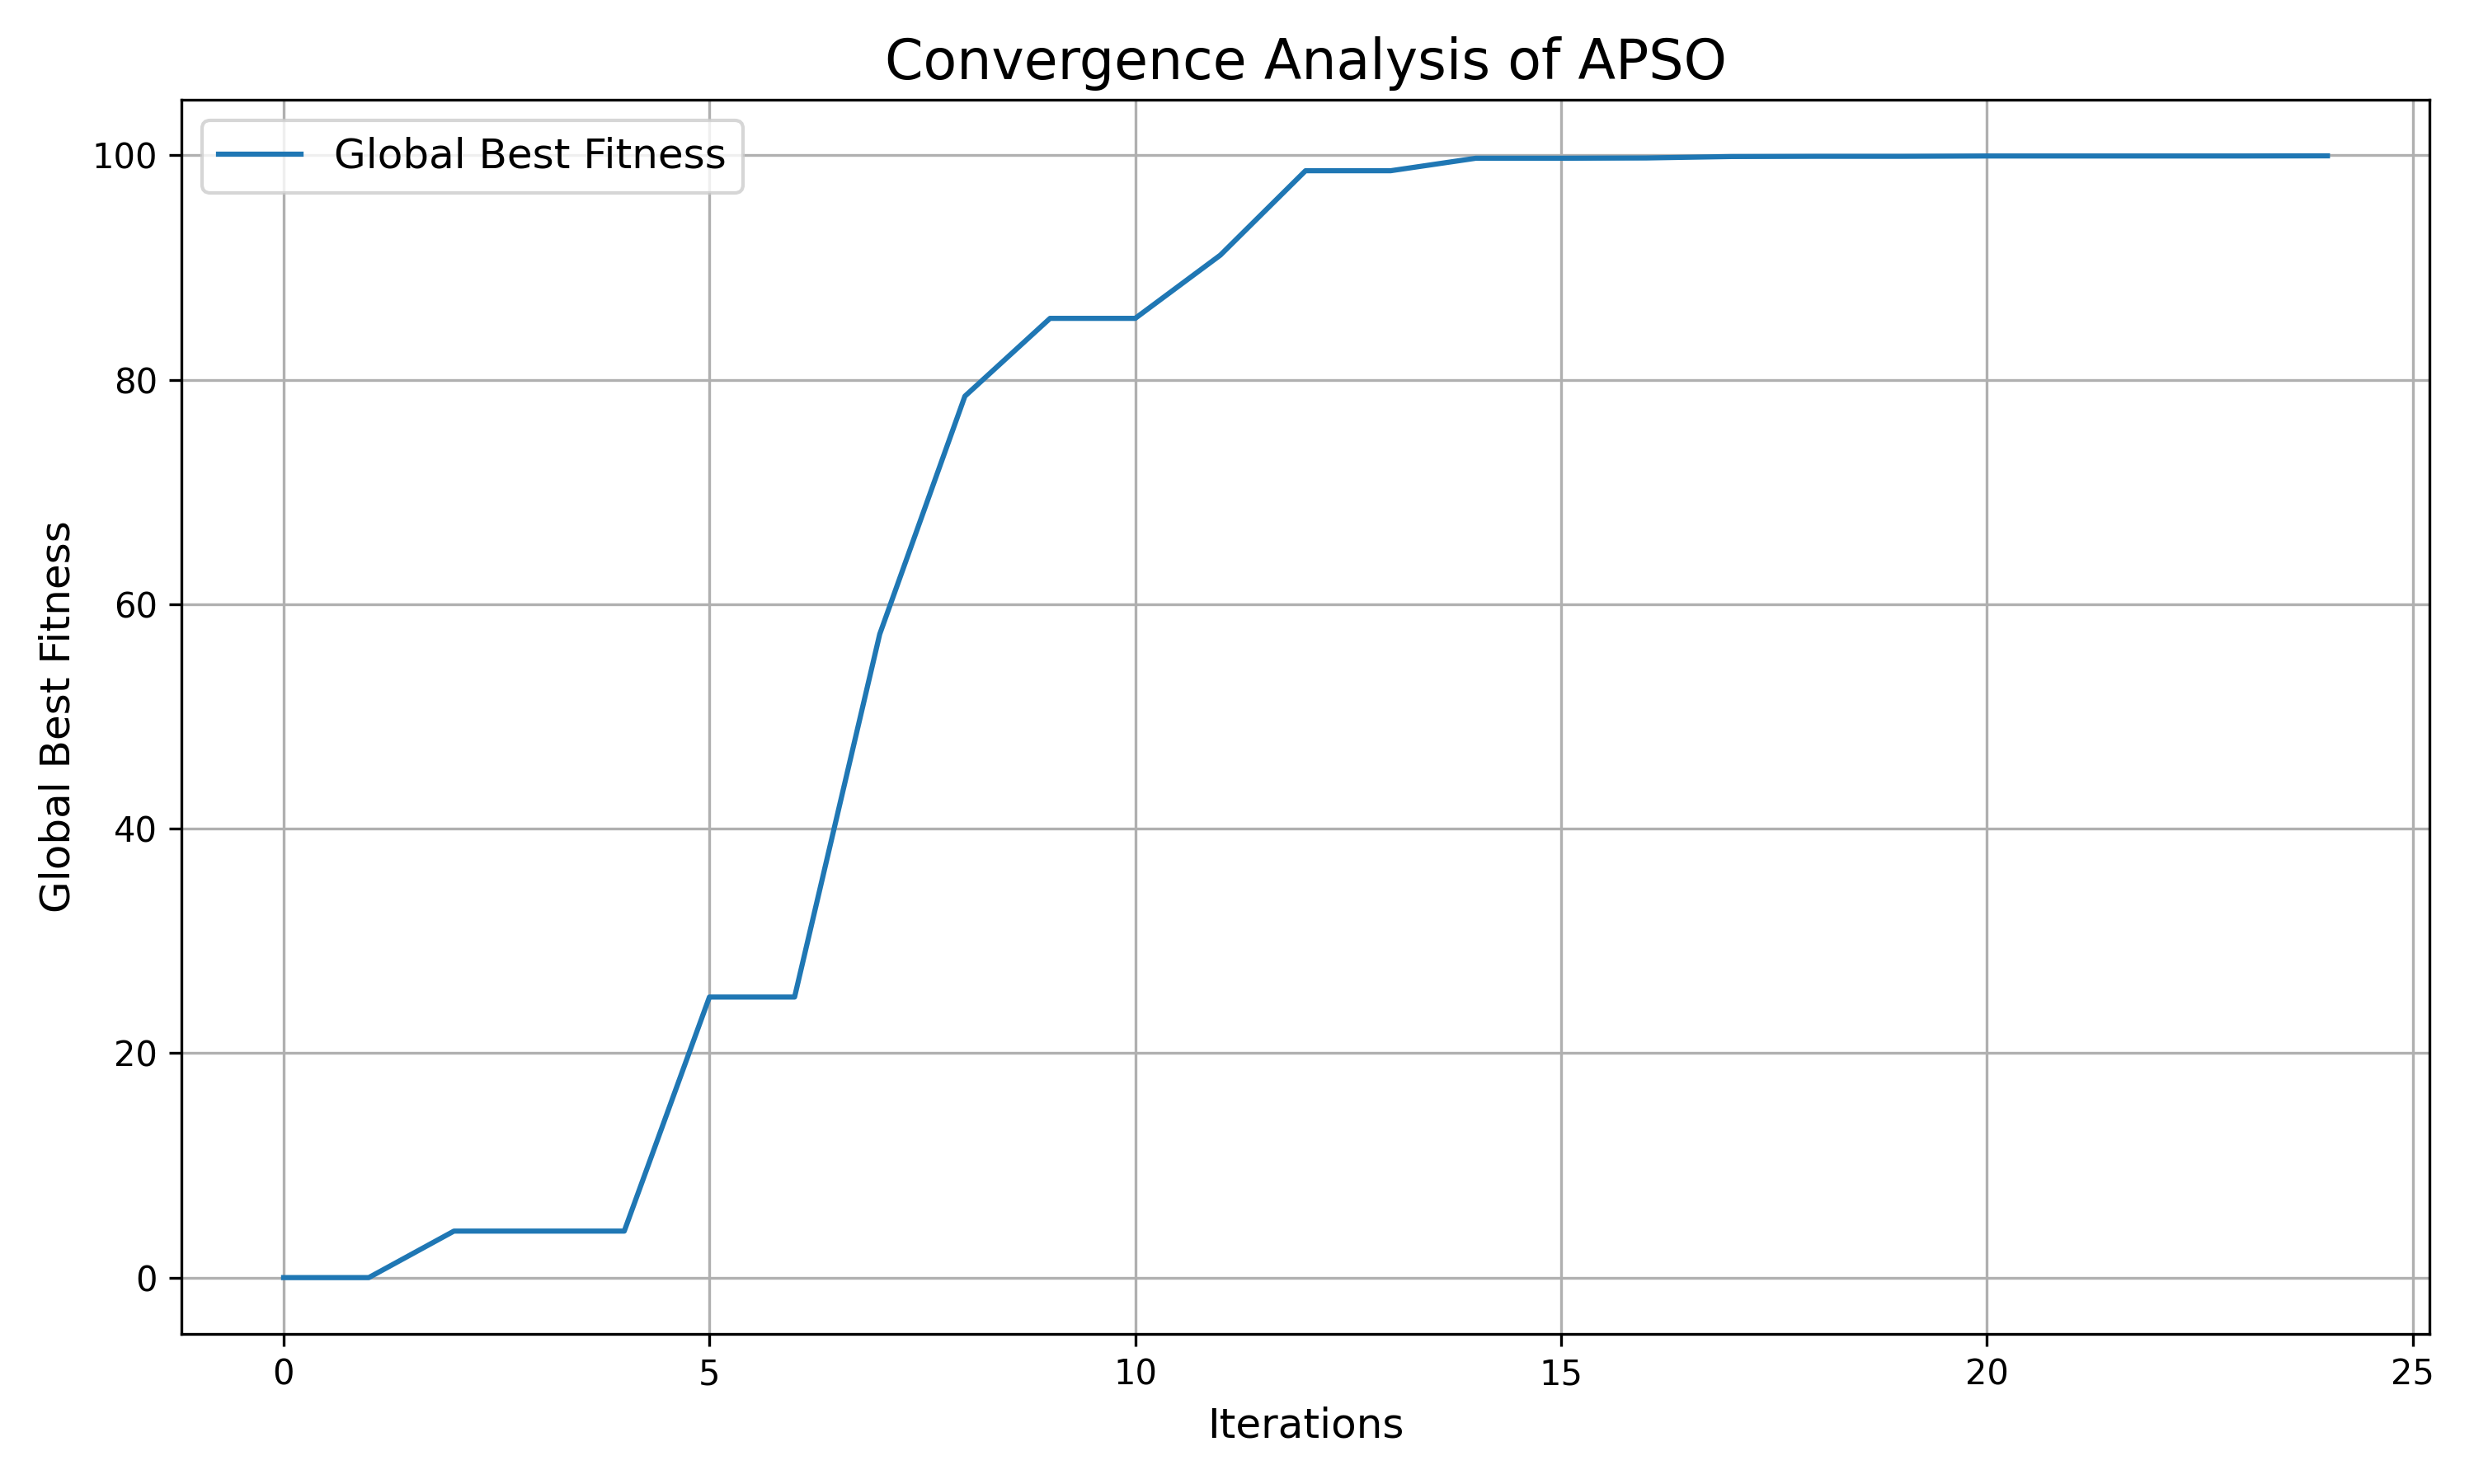
\includegraphics[width=\textwidth]{../plots/r2_without_noise/convergence_analysis.png}
            \caption{Convergence analysis}
        \end{subfigure}
        \caption{Source Seeking without Noise}
    \end{figure}
\end{frame}

% % % % ------------------------ Source Seeking with noise ------------------------
\begin{frame}{Source Seeking with noise}    
    \begin{figure}[h]
        \centering
        \begin{subfigure}[b]{0.32\textwidth}
            \centering
            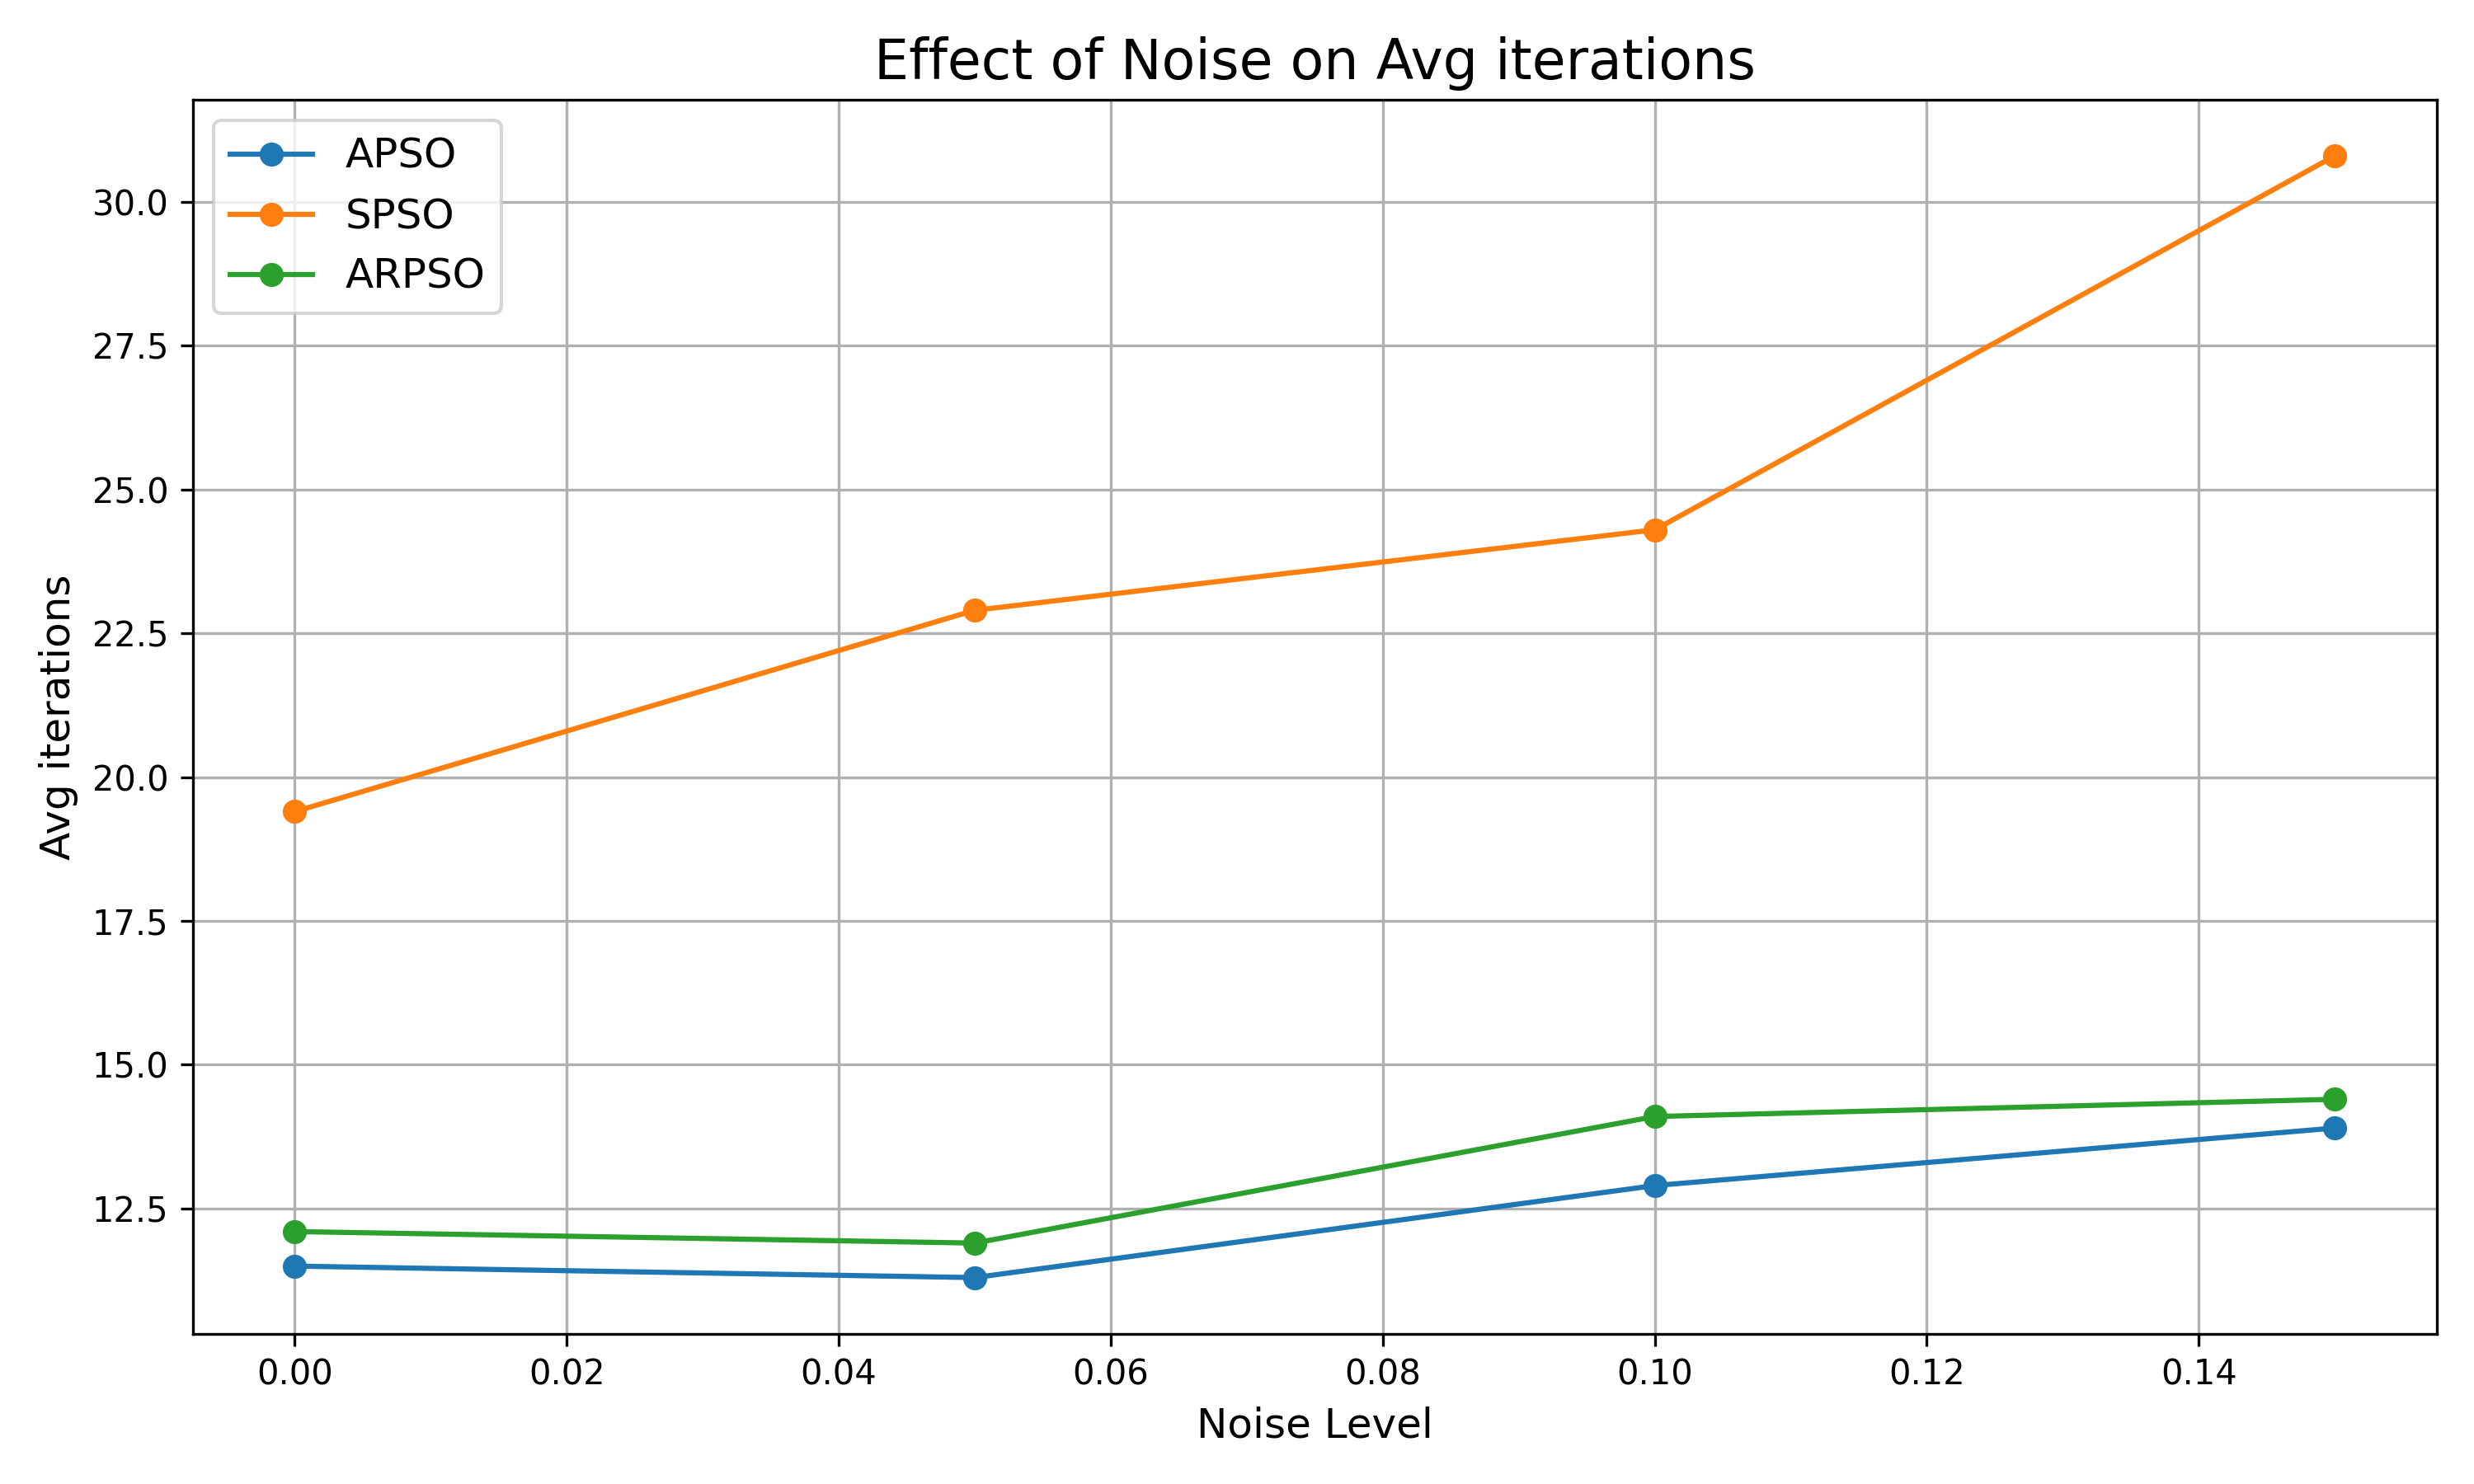
\includegraphics[width=\textwidth]{../plots/r1_with_noise/avg_iterations_vs_noise.png}
            \caption{iterations vs Noise}
        \end{subfigure}
        \hfill
        \begin{subfigure}[b]{0.32\textwidth}
            \centering
            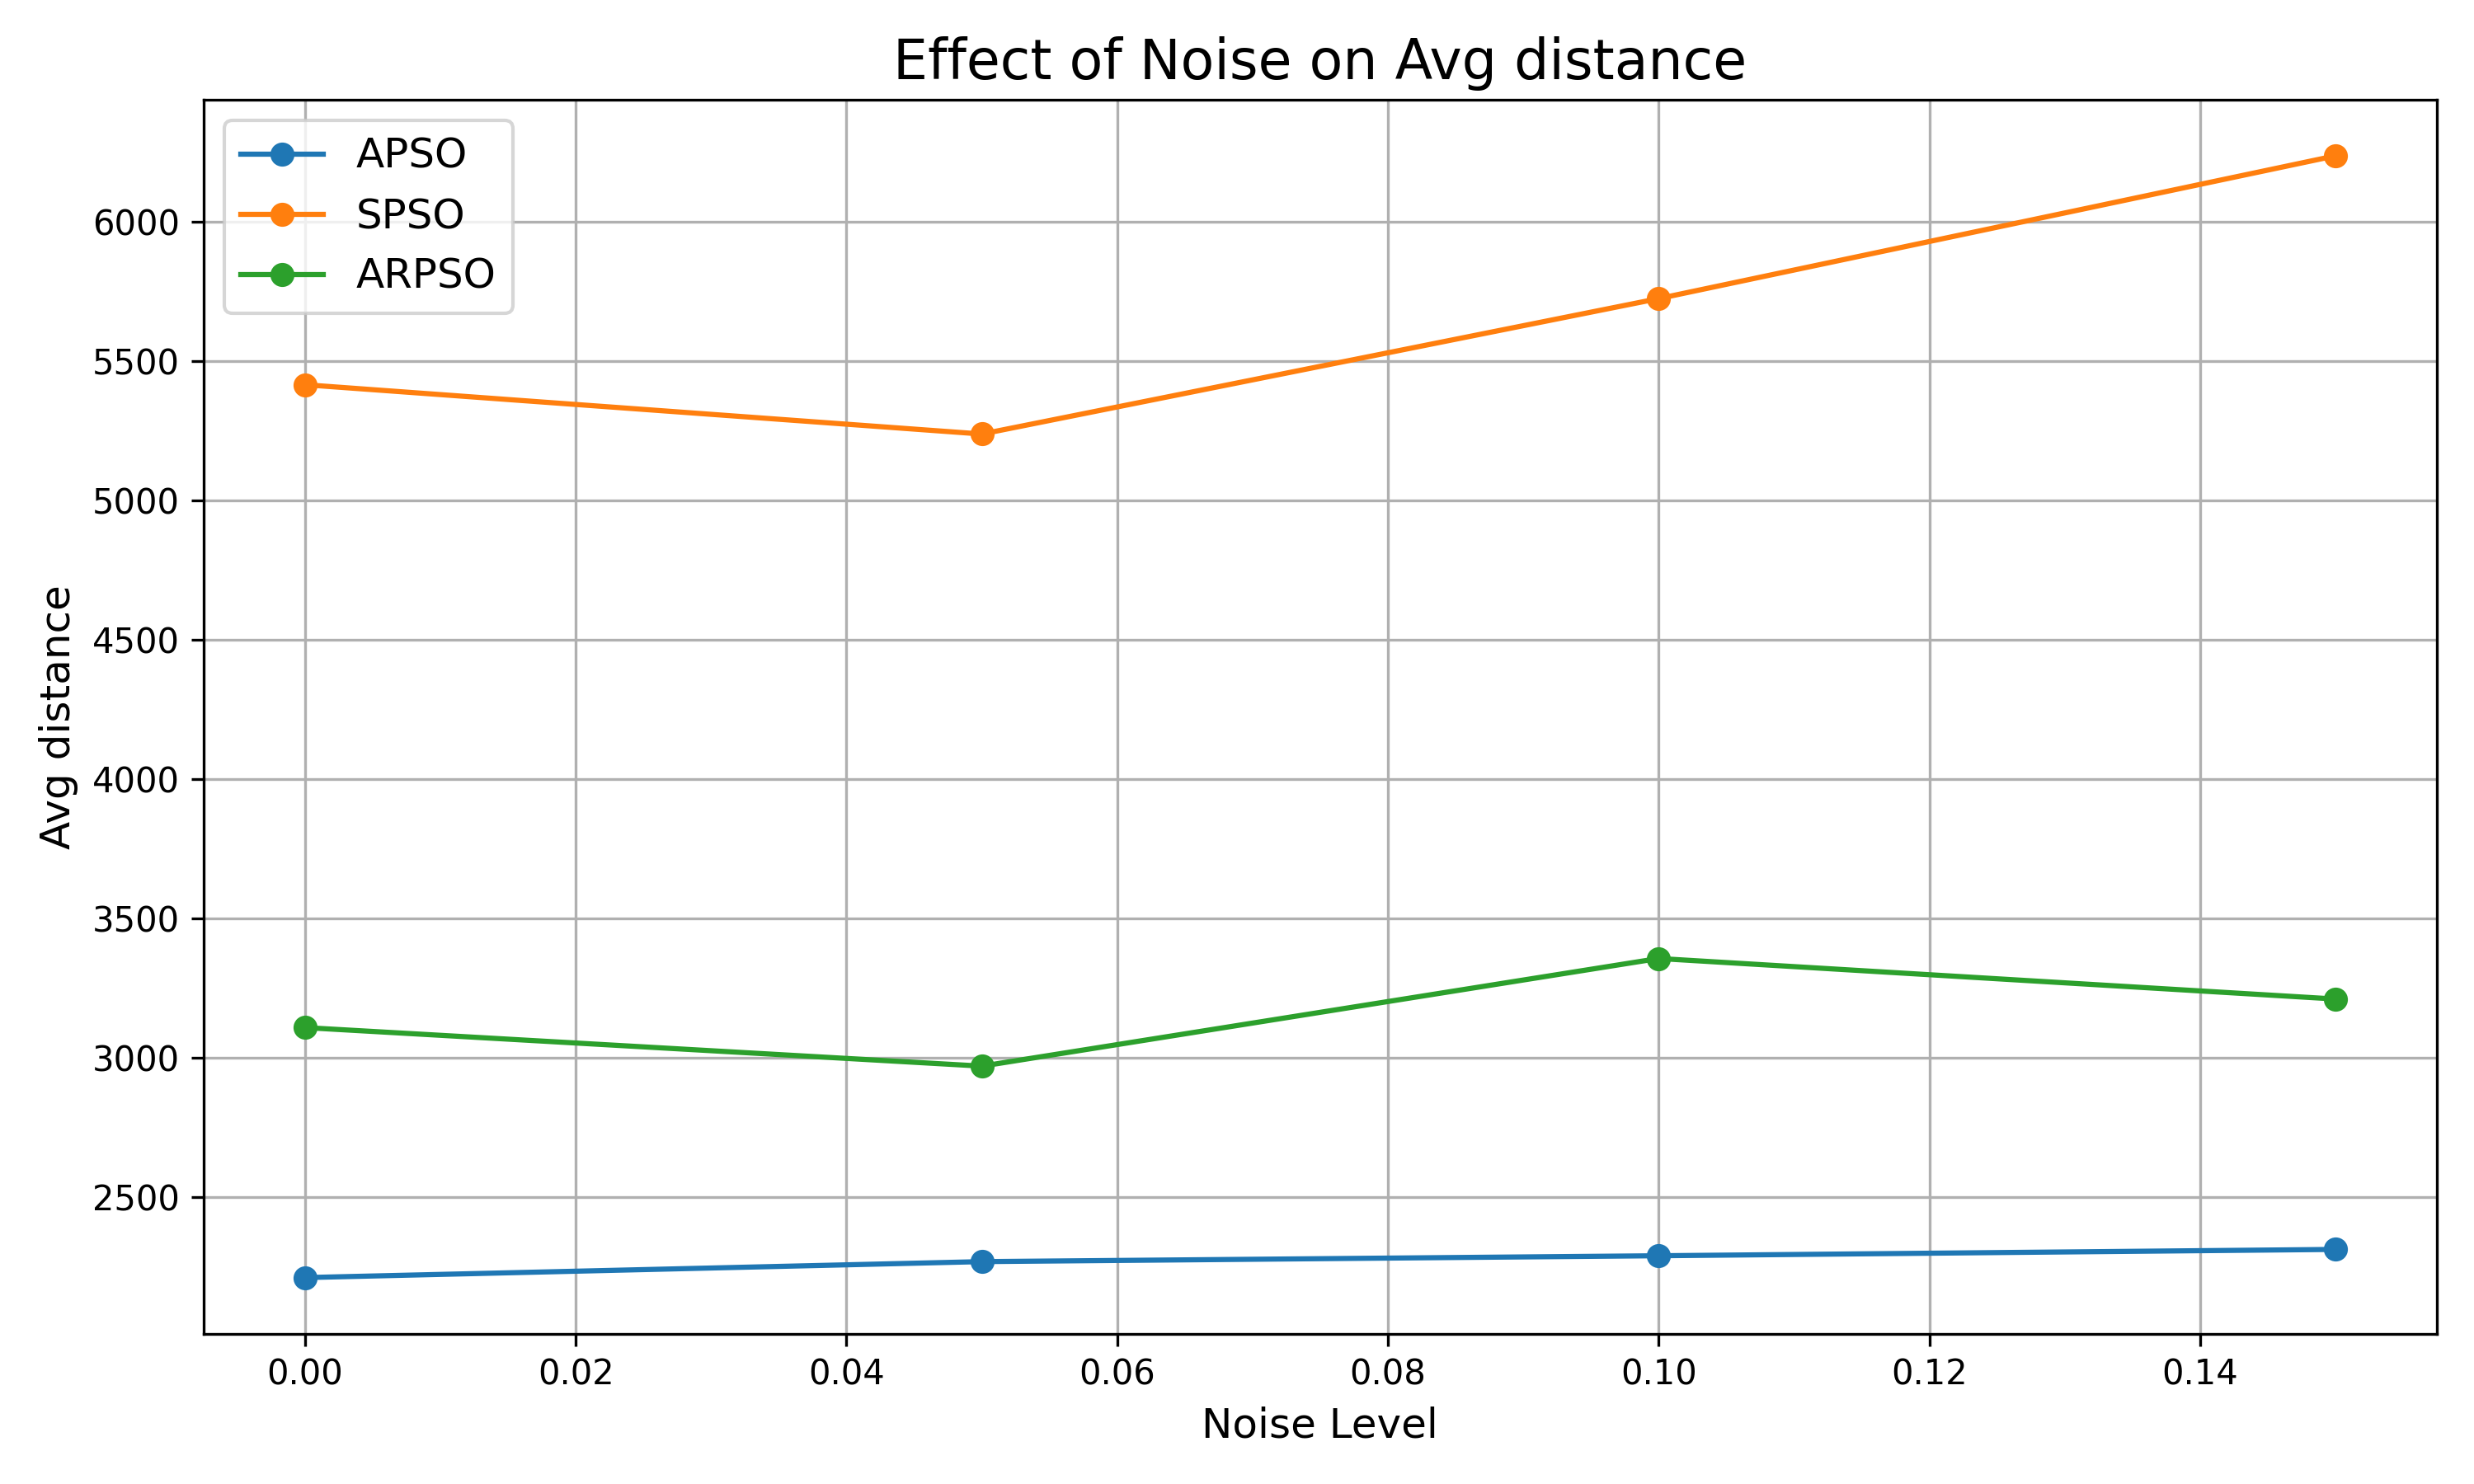
\includegraphics[width=\textwidth]{../plots/r1_with_noise/avg_distance_vs_noise.png}
            \caption{Distance vs Noise}
        \end{subfigure}
        \hfill
        \begin{subfigure}[b]{0.32\textwidth}
            \centering
            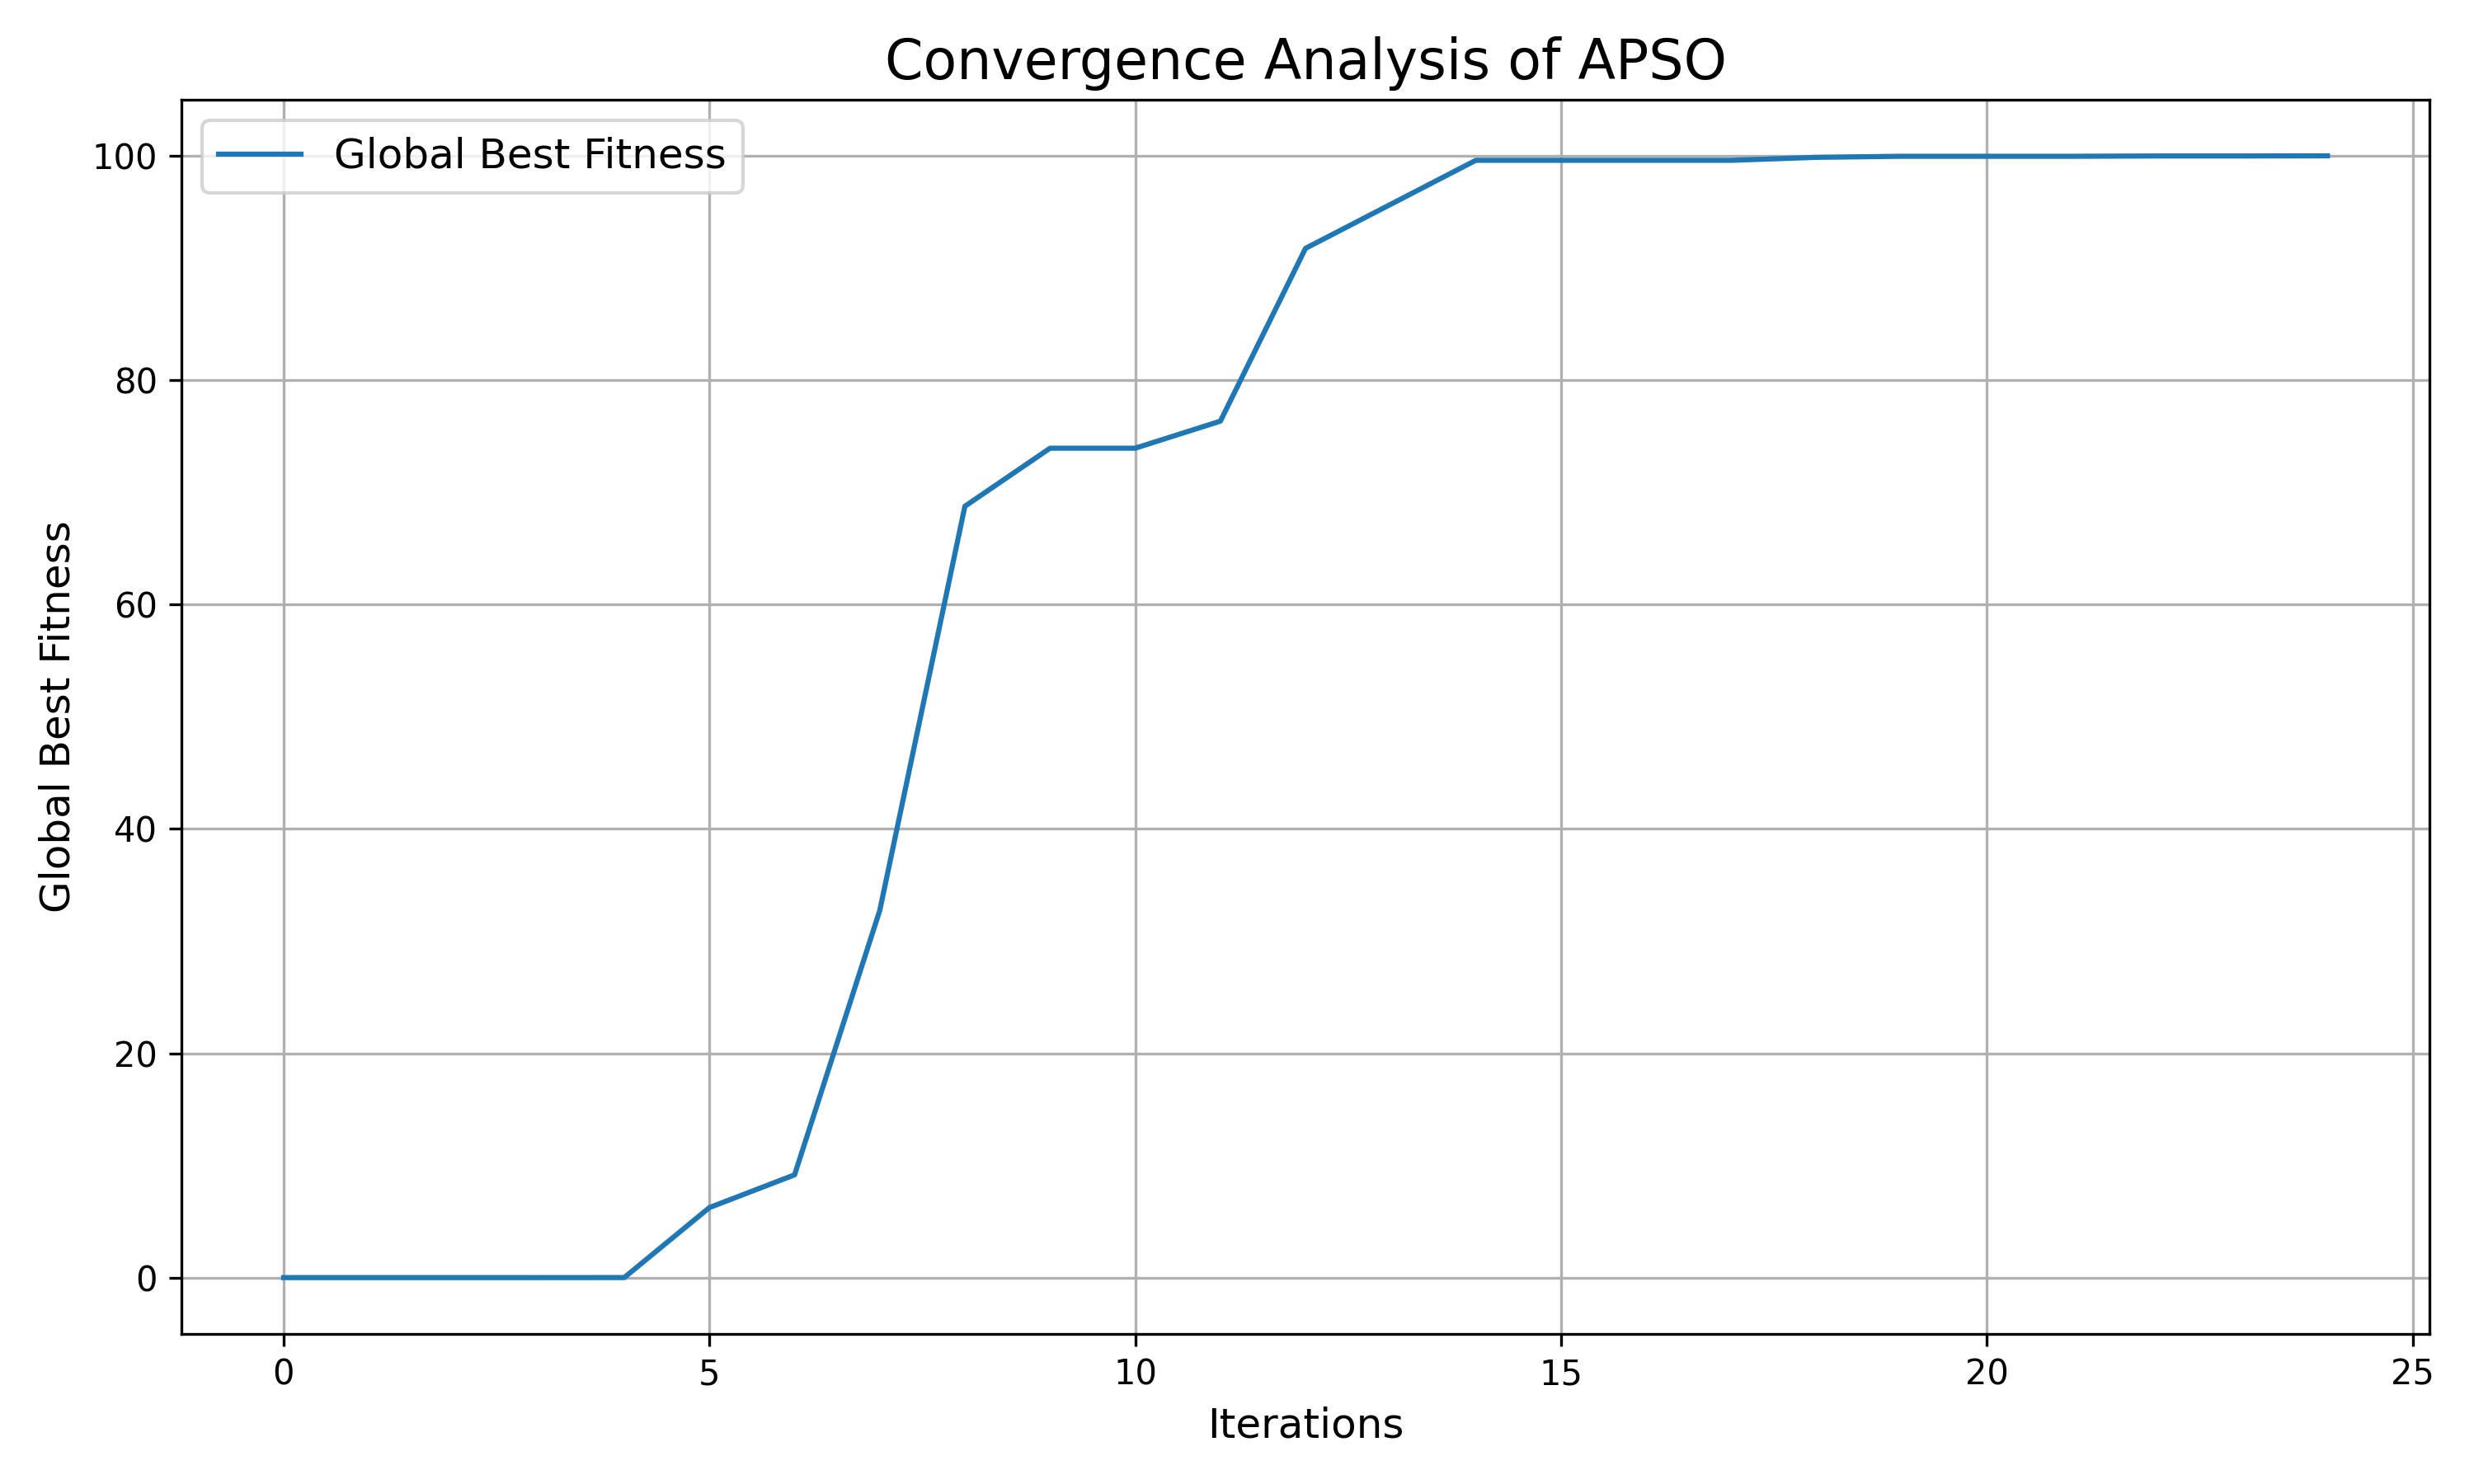
\includegraphics[width=\textwidth]{../plots/r1_with_noise/convergence_analysis.png}
            \caption{Convergence analysis}
        \end{subfigure}
        \caption{Source Seeking with Noise for 30 UAV's}
    \end{figure}
\end{frame}

% % % % ------------------------ Source Seeking Analysis ------------------------
\begin{frame}{Source Seeking Conclusions}    
    \begin{itemize}
        \item APSO consistently outperforms both SPSO and ARPSO across all noise levels.
        \begin{itemize}
            \item APSO requires fewer iterations
            \item APSO travels less distance
        \end{itemize}
        \item APSO shows the best scaling as UAV count increases, iterations actually decrease and SPSO shows the worst scaling in terms of distance traveled.
        \item All algorithms show degraded performance as noise increases
        \begin{itemize}
            \item The number of iterations increases with noise level
            \item The distance traveled also generally increases with noise level
        \end{itemize}
        \item APSO shows the best robustness to noise
        \begin{itemize}
            \item The slope of the APSO line is less steep than SPSO, indicating better resilience to noise
            \item Even at $0.15$ noise level, APSO maintains good performance
        \end{itemize}
        \item APSO provides smoother convergence under noise. As its acceleration based approach allows it to maintain momentum through noisy measurements, while the standard PSO gets easily misled by noise.
    \end{itemize}
\end{frame}

% % % % ------------------------ CEC 2022 ------------------------
\begin{frame}{CEC'22 Benchmark Suit}
    \textbf{What are CEC Benchmarks?} \\
    \begin{itemize}
        \item Standard test suite developed by IEEE Congress on Evolutionary Computation
        \item CEC 2022 includes diverse optimization problems with known properties
        \item Designed to rigorously evaluate and compare optimization algorithms\\
    \end{itemize}

    \textbf{Functions Implemented:} \\
    \begin{itemize}
        \item \textbf{F1 (Zakharov):} Continuous unimodal function with interdependent variables
        \item \textbf{F2 (Rosenbrock):} Continuous function with narrow curved valley
        \item \textbf{F3 (Schaffer):} Highly multimodal function with many local optima
        \item \textbf{F4 (Step Rastrigin):} Discontinuous multimodal function with plateaus
        \item \textbf{F5 (Levy):} Multimodal function with many local minima
    \end{itemize}
\end{frame}
\begin{frame}
    \textbf{Why these functions??}
    \begin{itemize}
        \item Represent diverse optimization challenges
        \item \textbf{F1-F2:} Test convergence precision and speed
        \item \textbf{F3-F5:} Test ability to escape local optima
        \item Combination reveals which hybrid approaches excel in different scenarios
    \end{itemize}
\end{frame}

\begin{frame}{CEC'22 Visualization}
    \centering
    \begin{figure}
        \centering
        % First row
        \begin{subfigure}[b]{0.19\textwidth}
            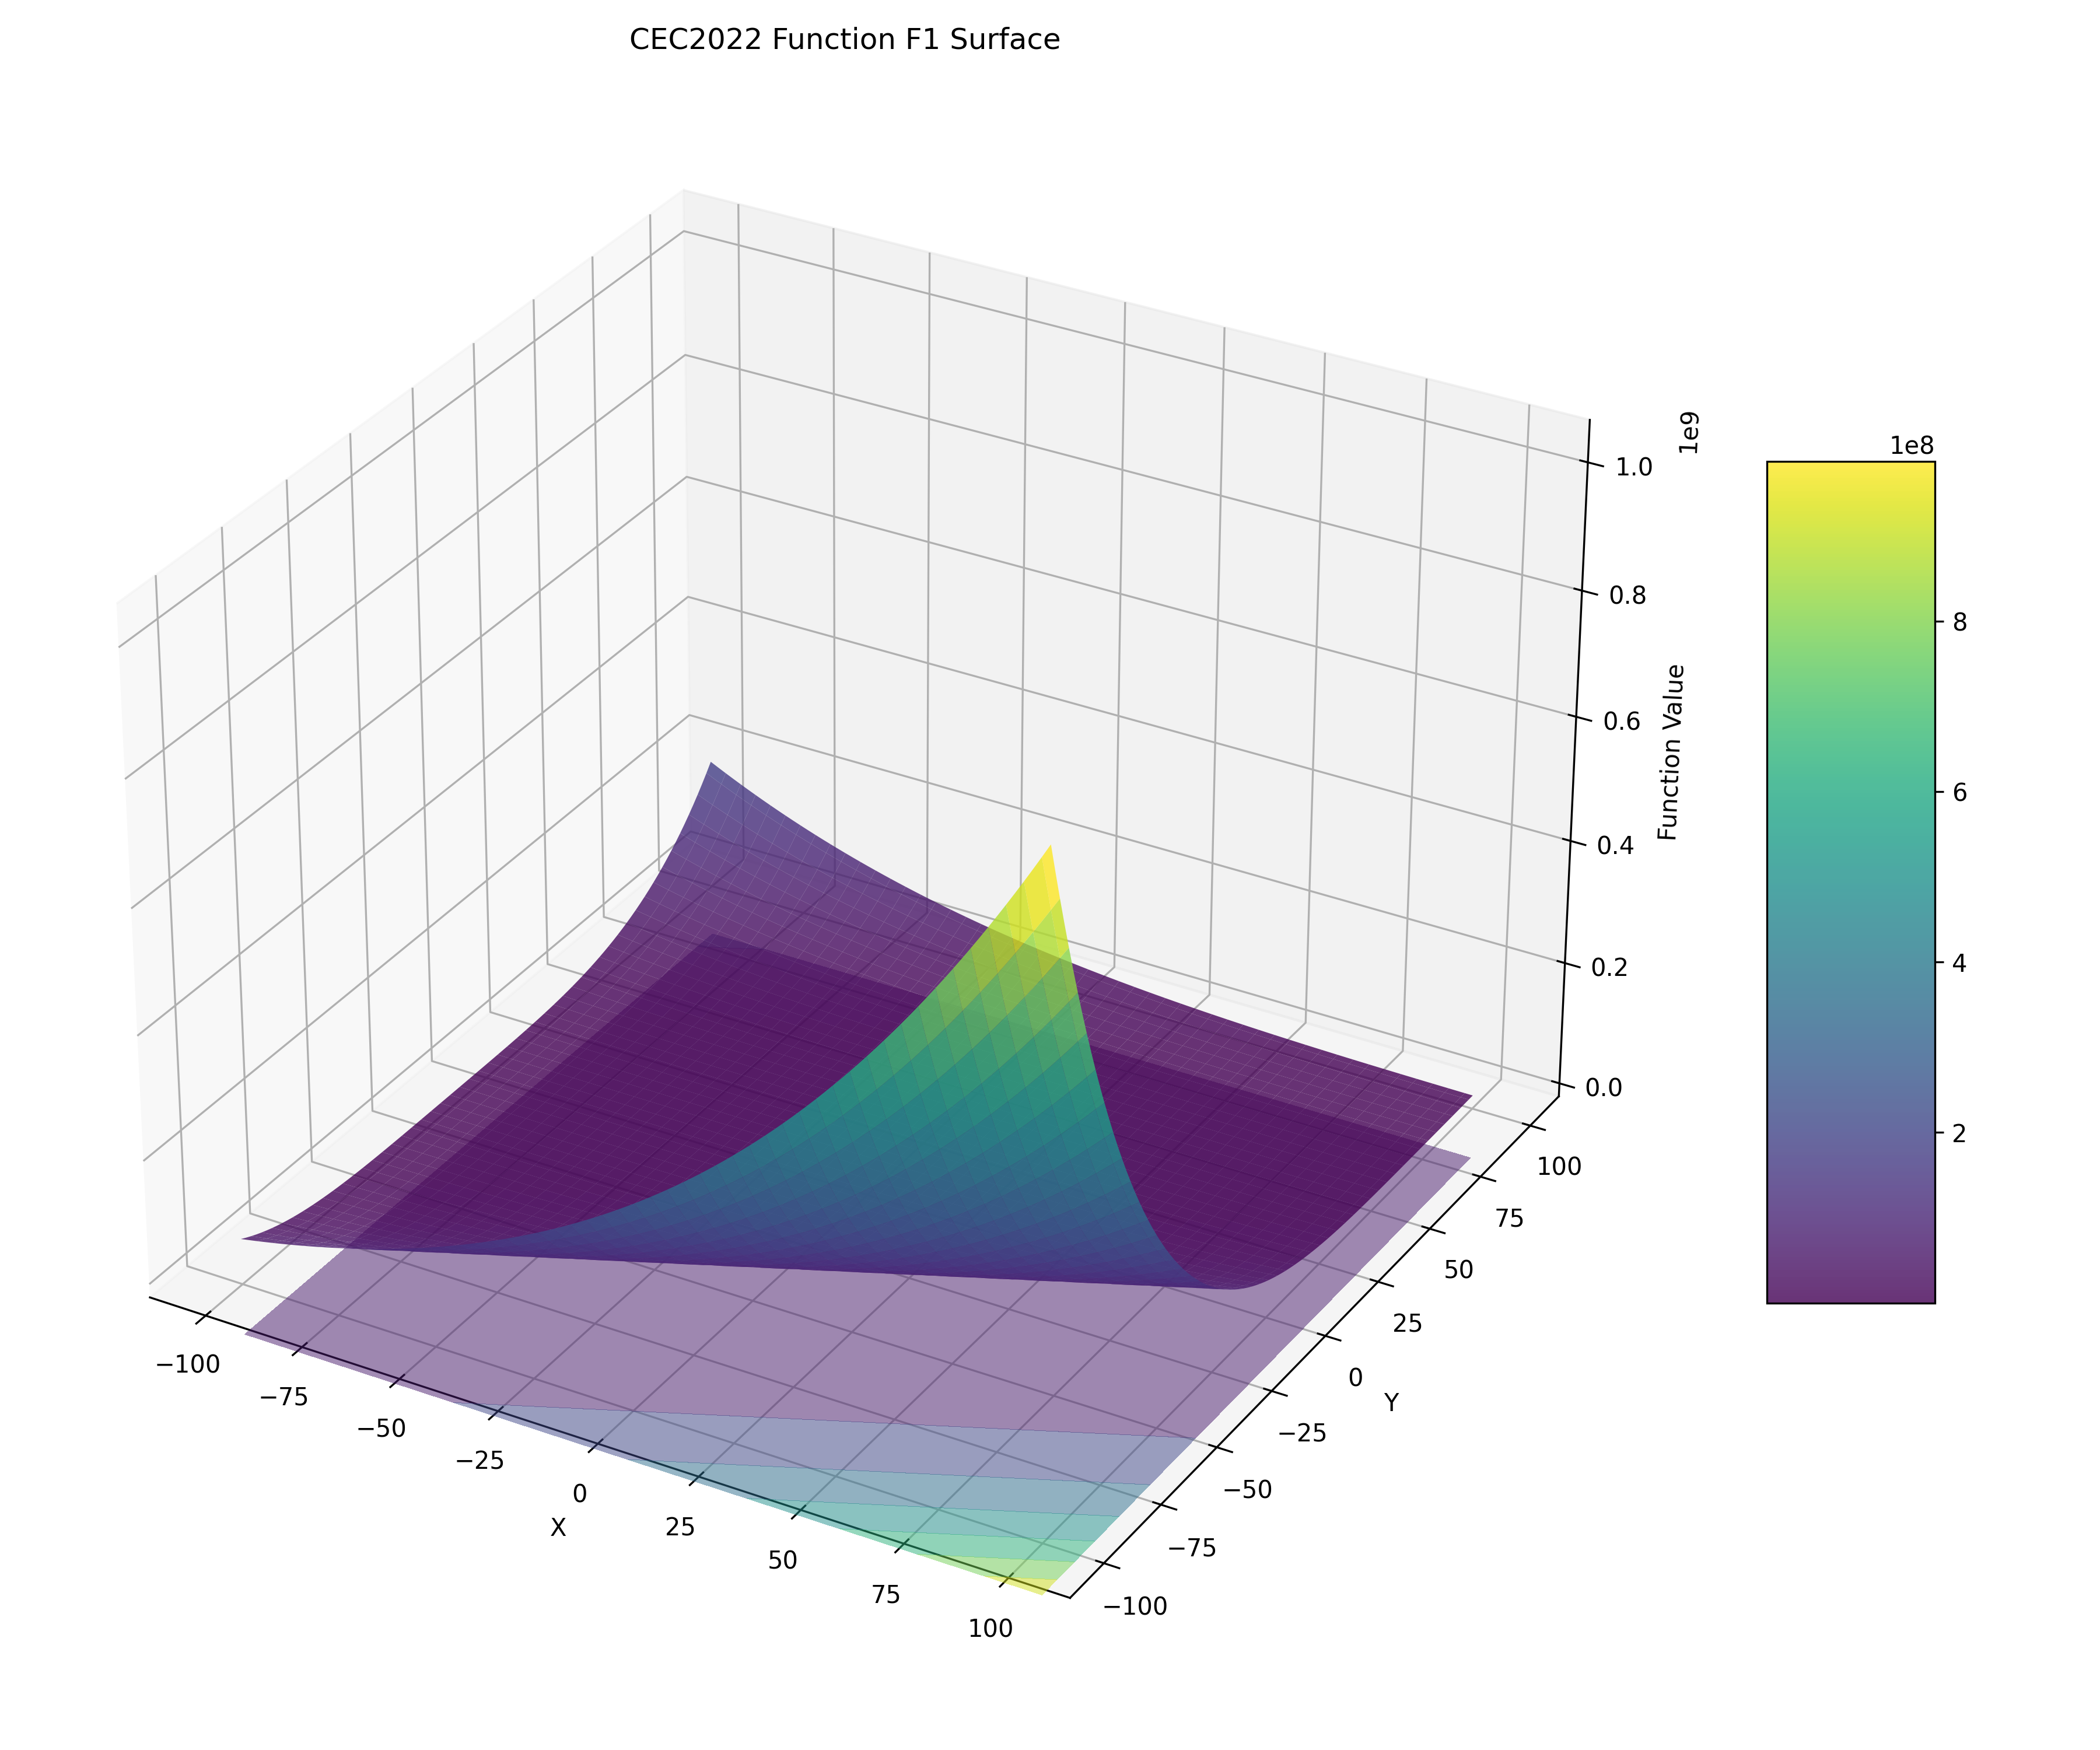
\includegraphics[width=\textwidth]{../plots/cec_bench/function_surface_f1.png}
            \caption*{F1}
        \end{subfigure}
        \hfill
        \begin{subfigure}[b]{0.19\textwidth}
            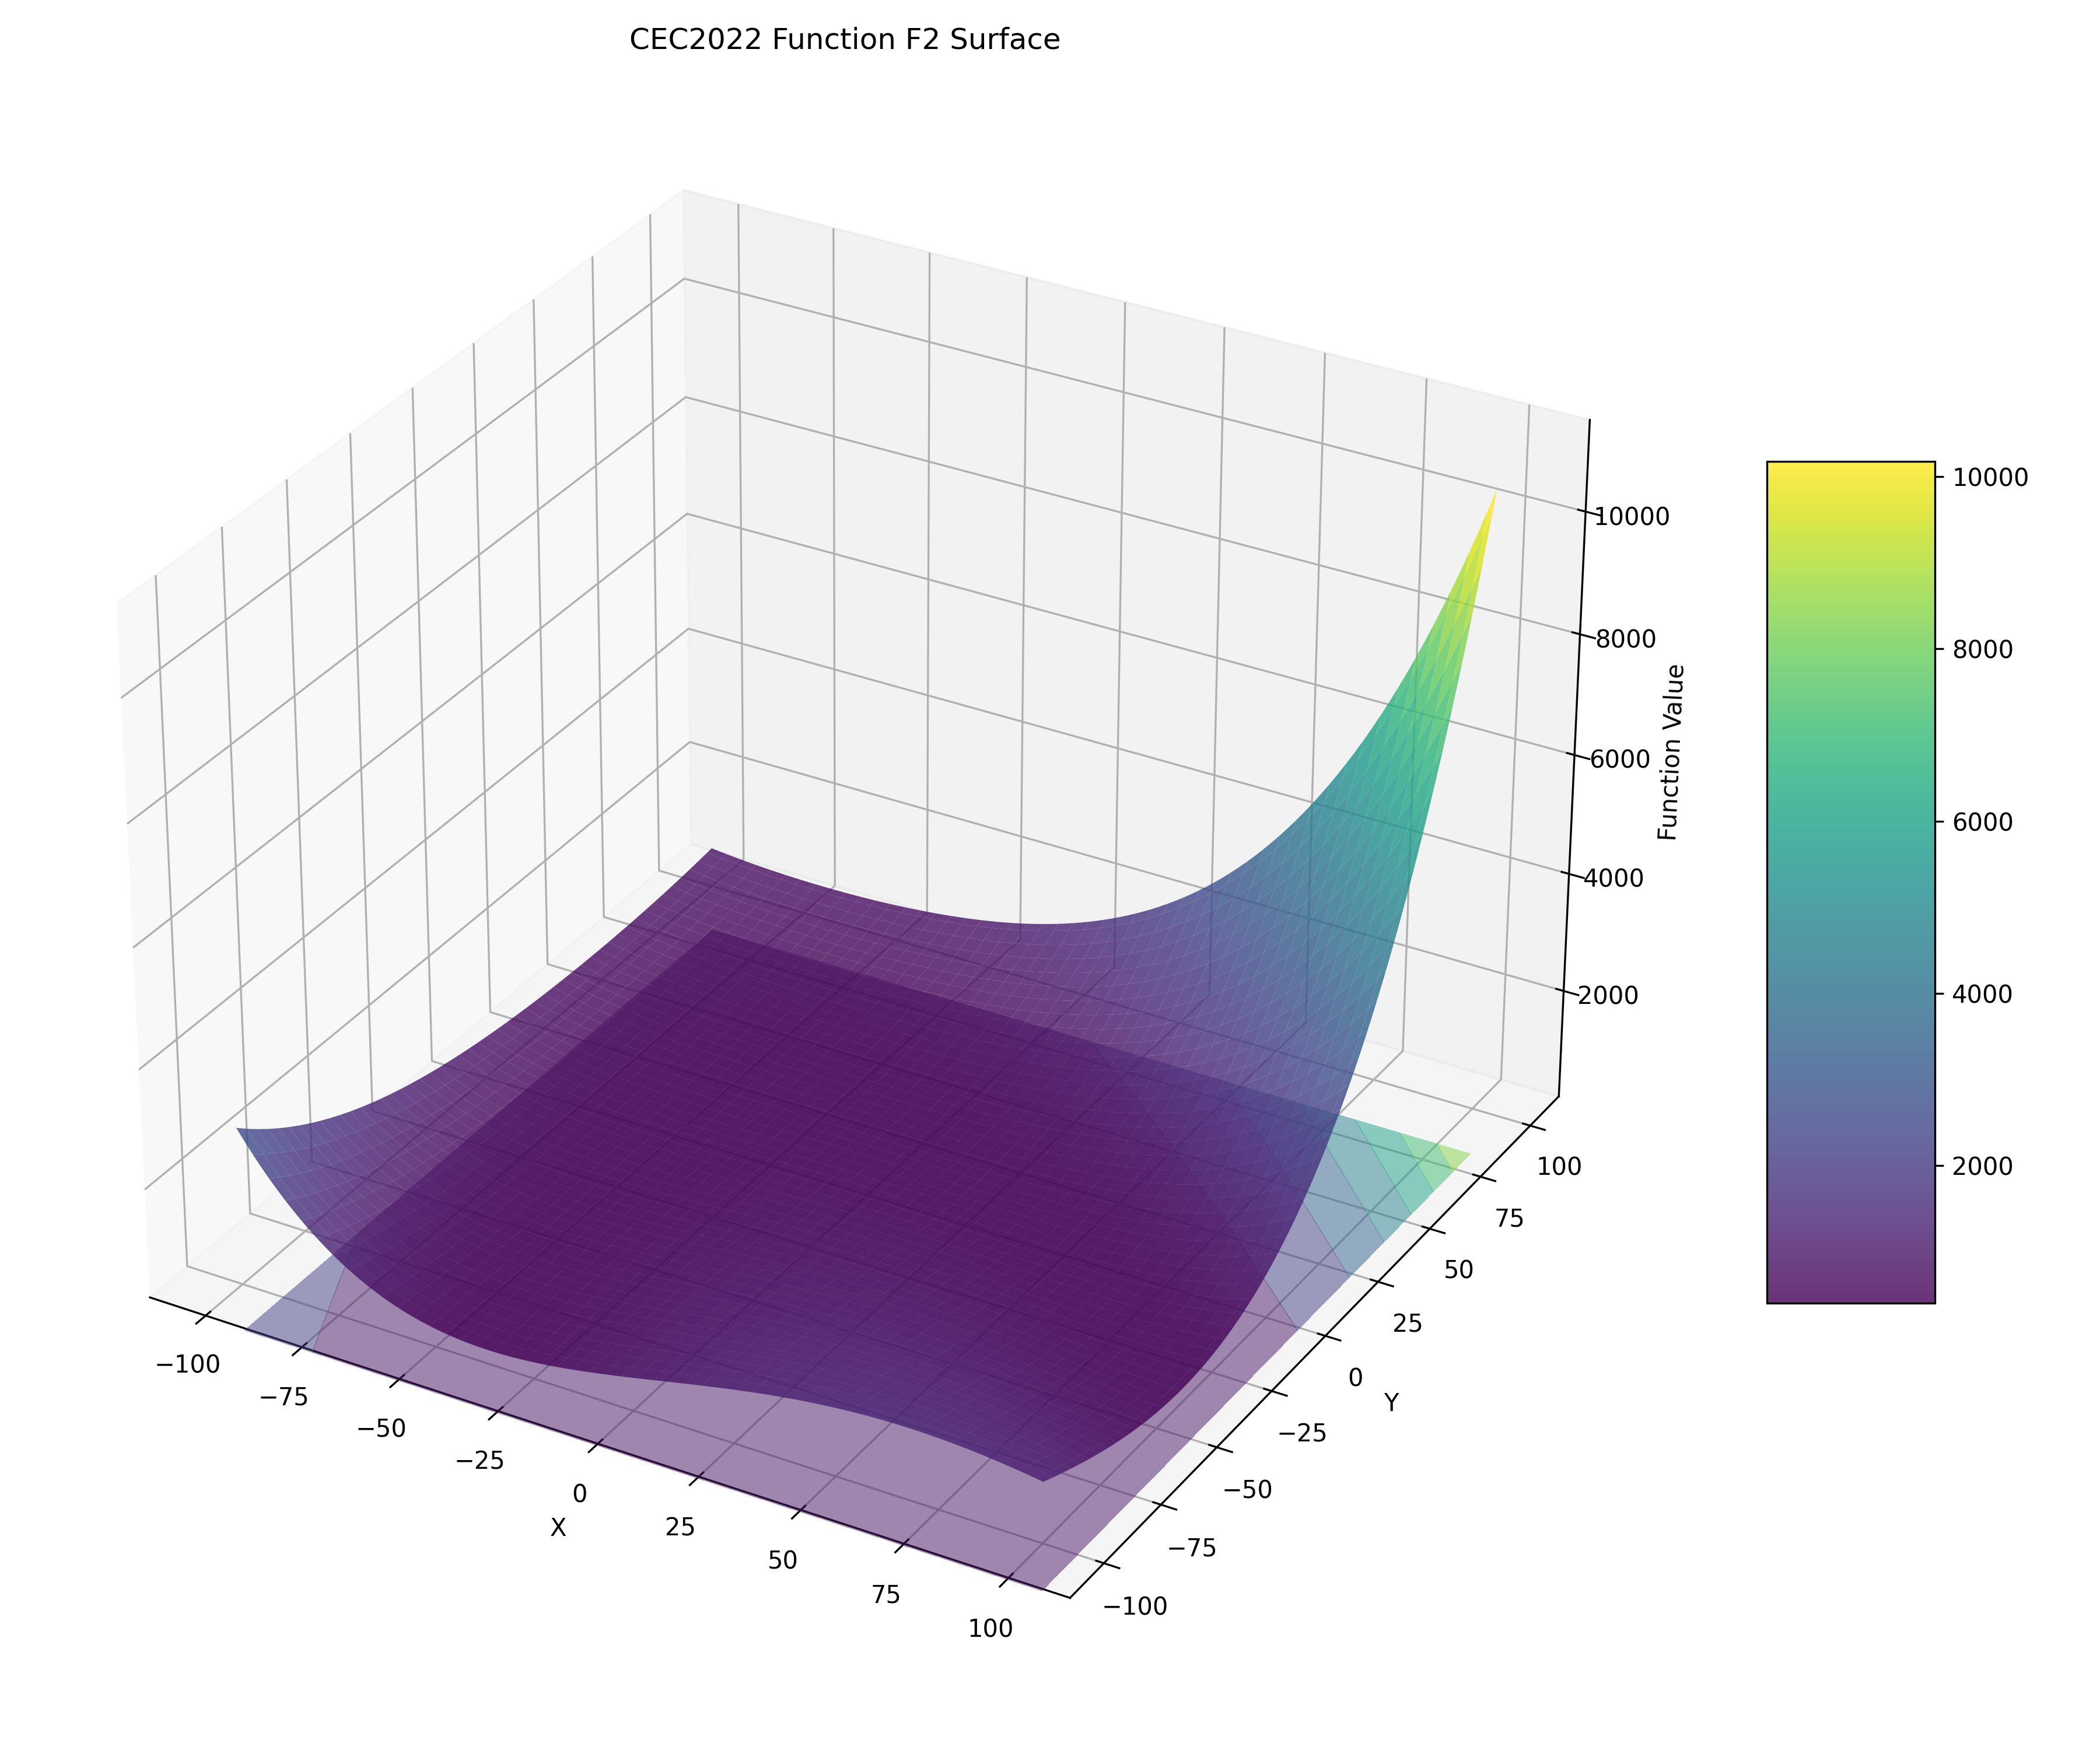
\includegraphics[width=\textwidth]{../plots/cec_bench/function_surface_f2.png}
            \caption*{F2}
        \end{subfigure}
        \hfill
        \begin{subfigure}[b]{0.19\textwidth}
            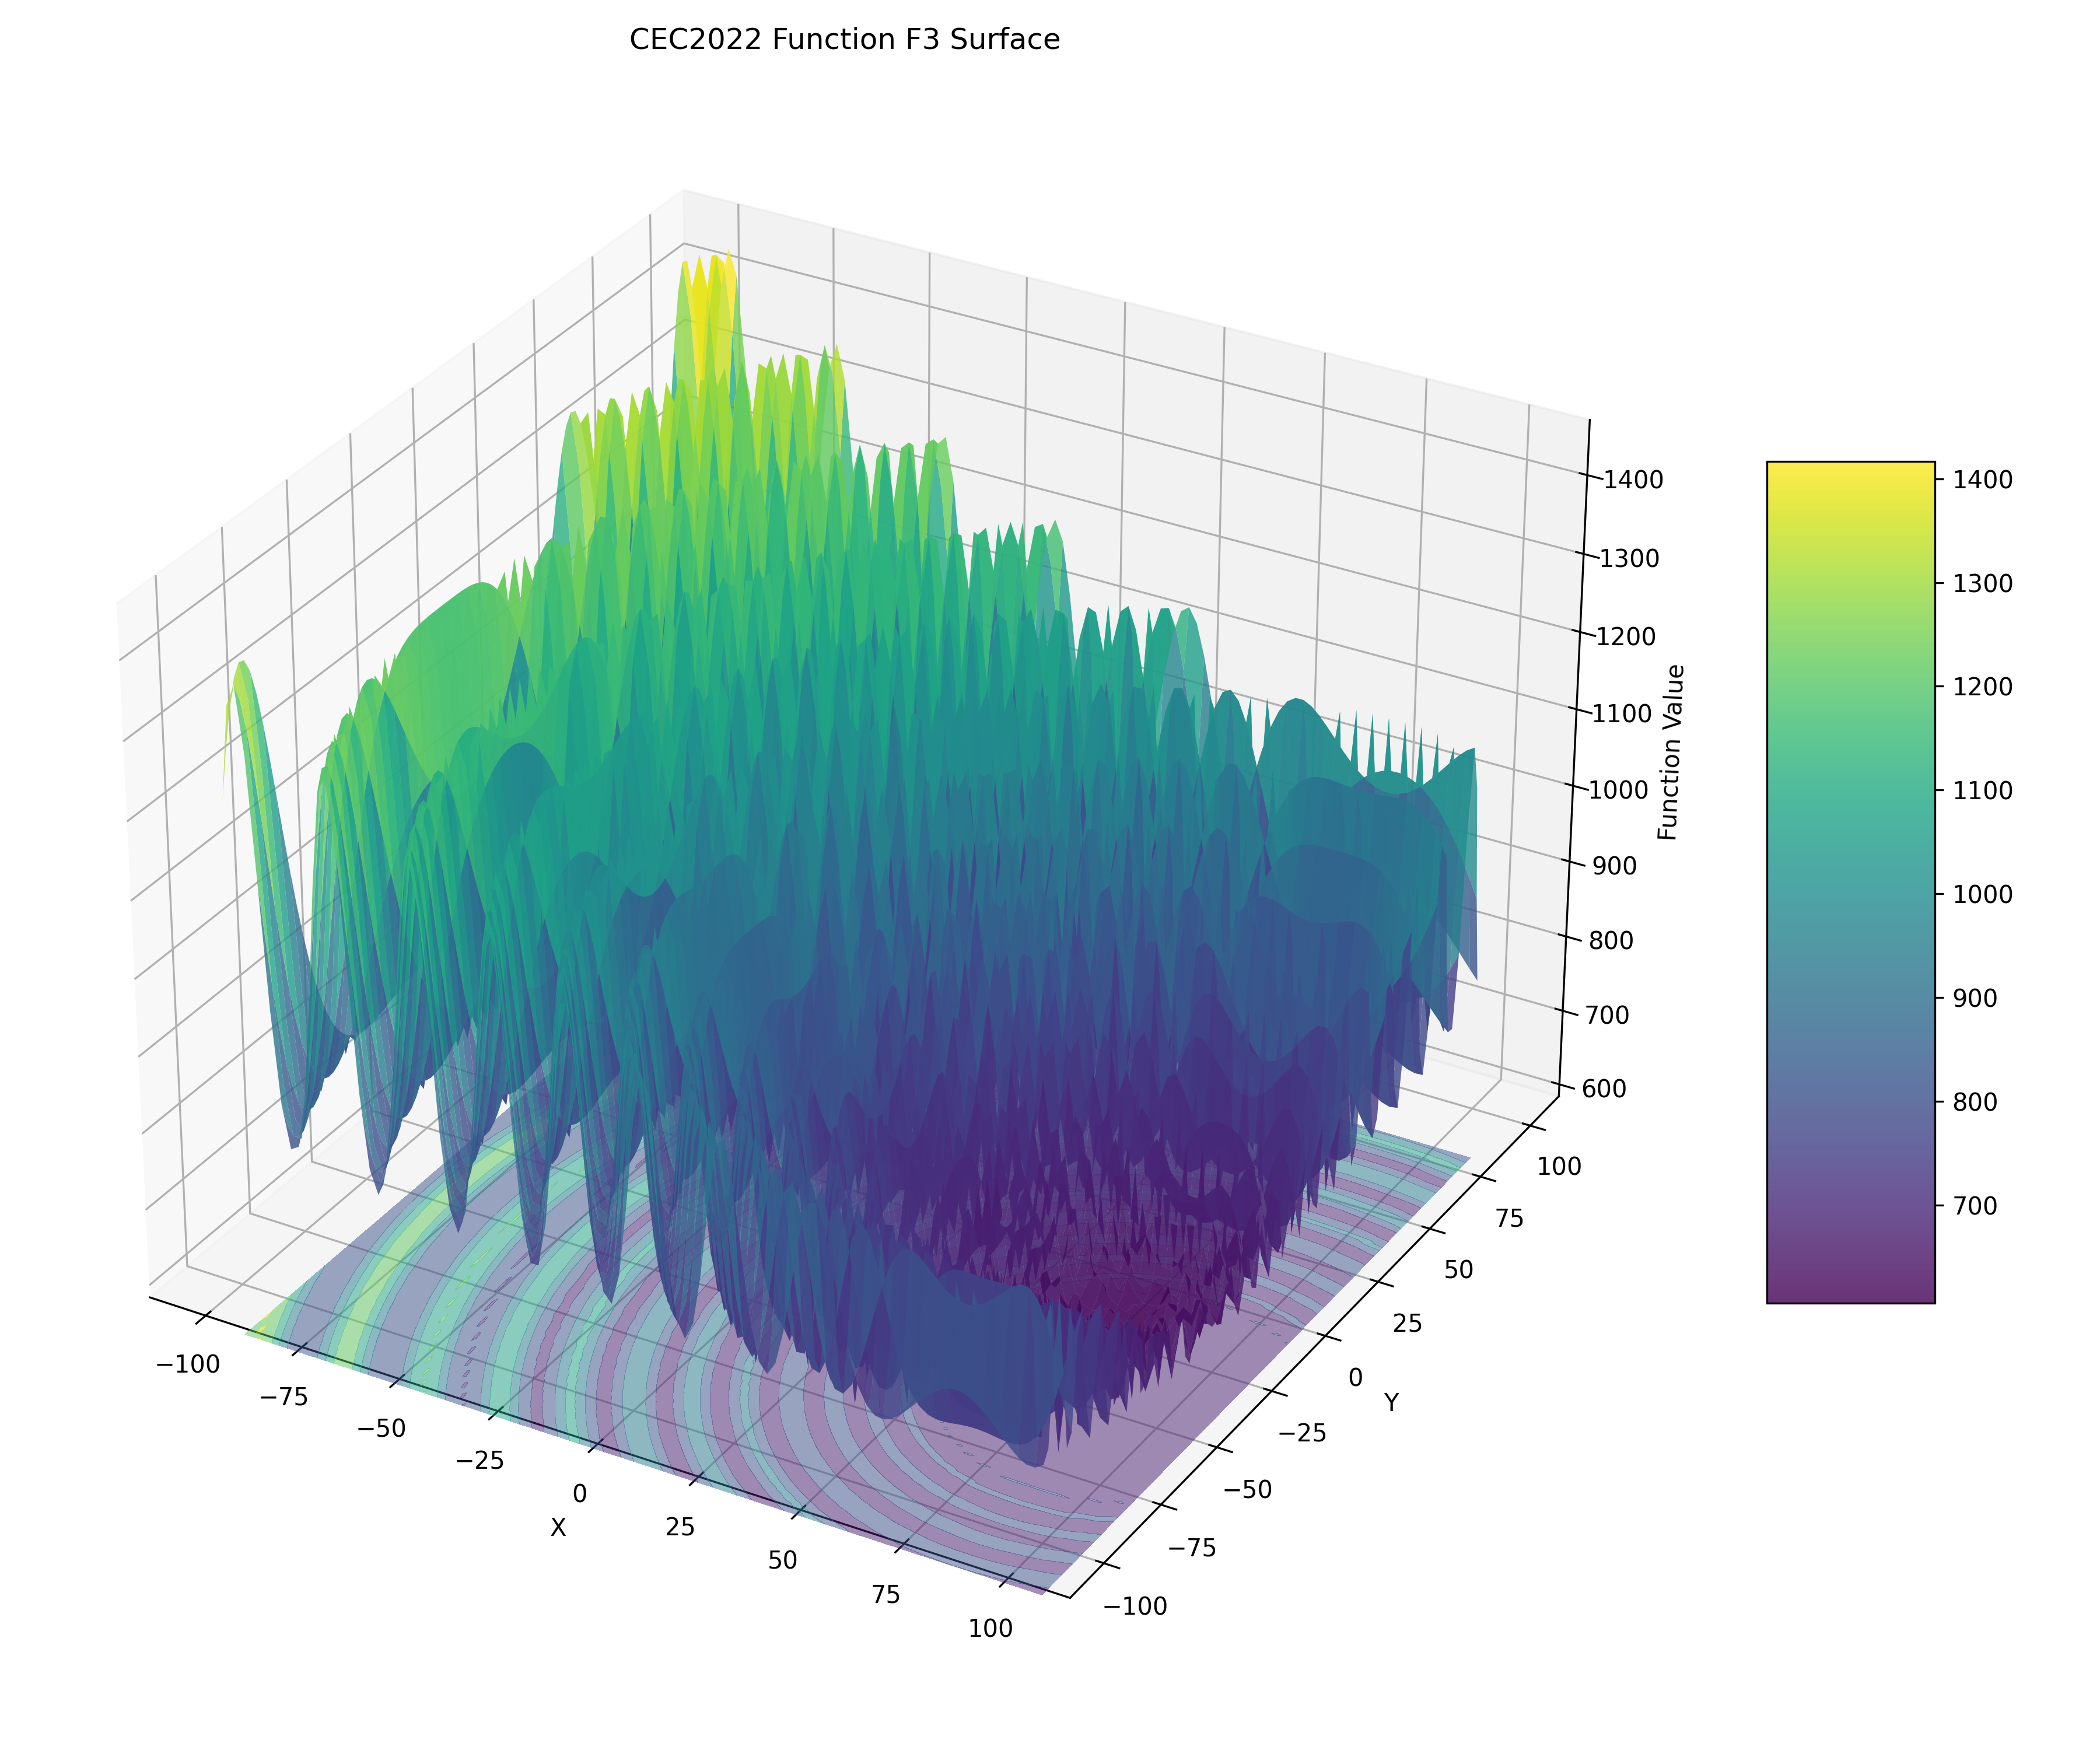
\includegraphics[width=\textwidth]{../plots/cec_bench/function_surface_f3.png}
            \caption*{F3}
        \end{subfigure}
        \hfill
        \begin{subfigure}[b]{0.19\textwidth}
            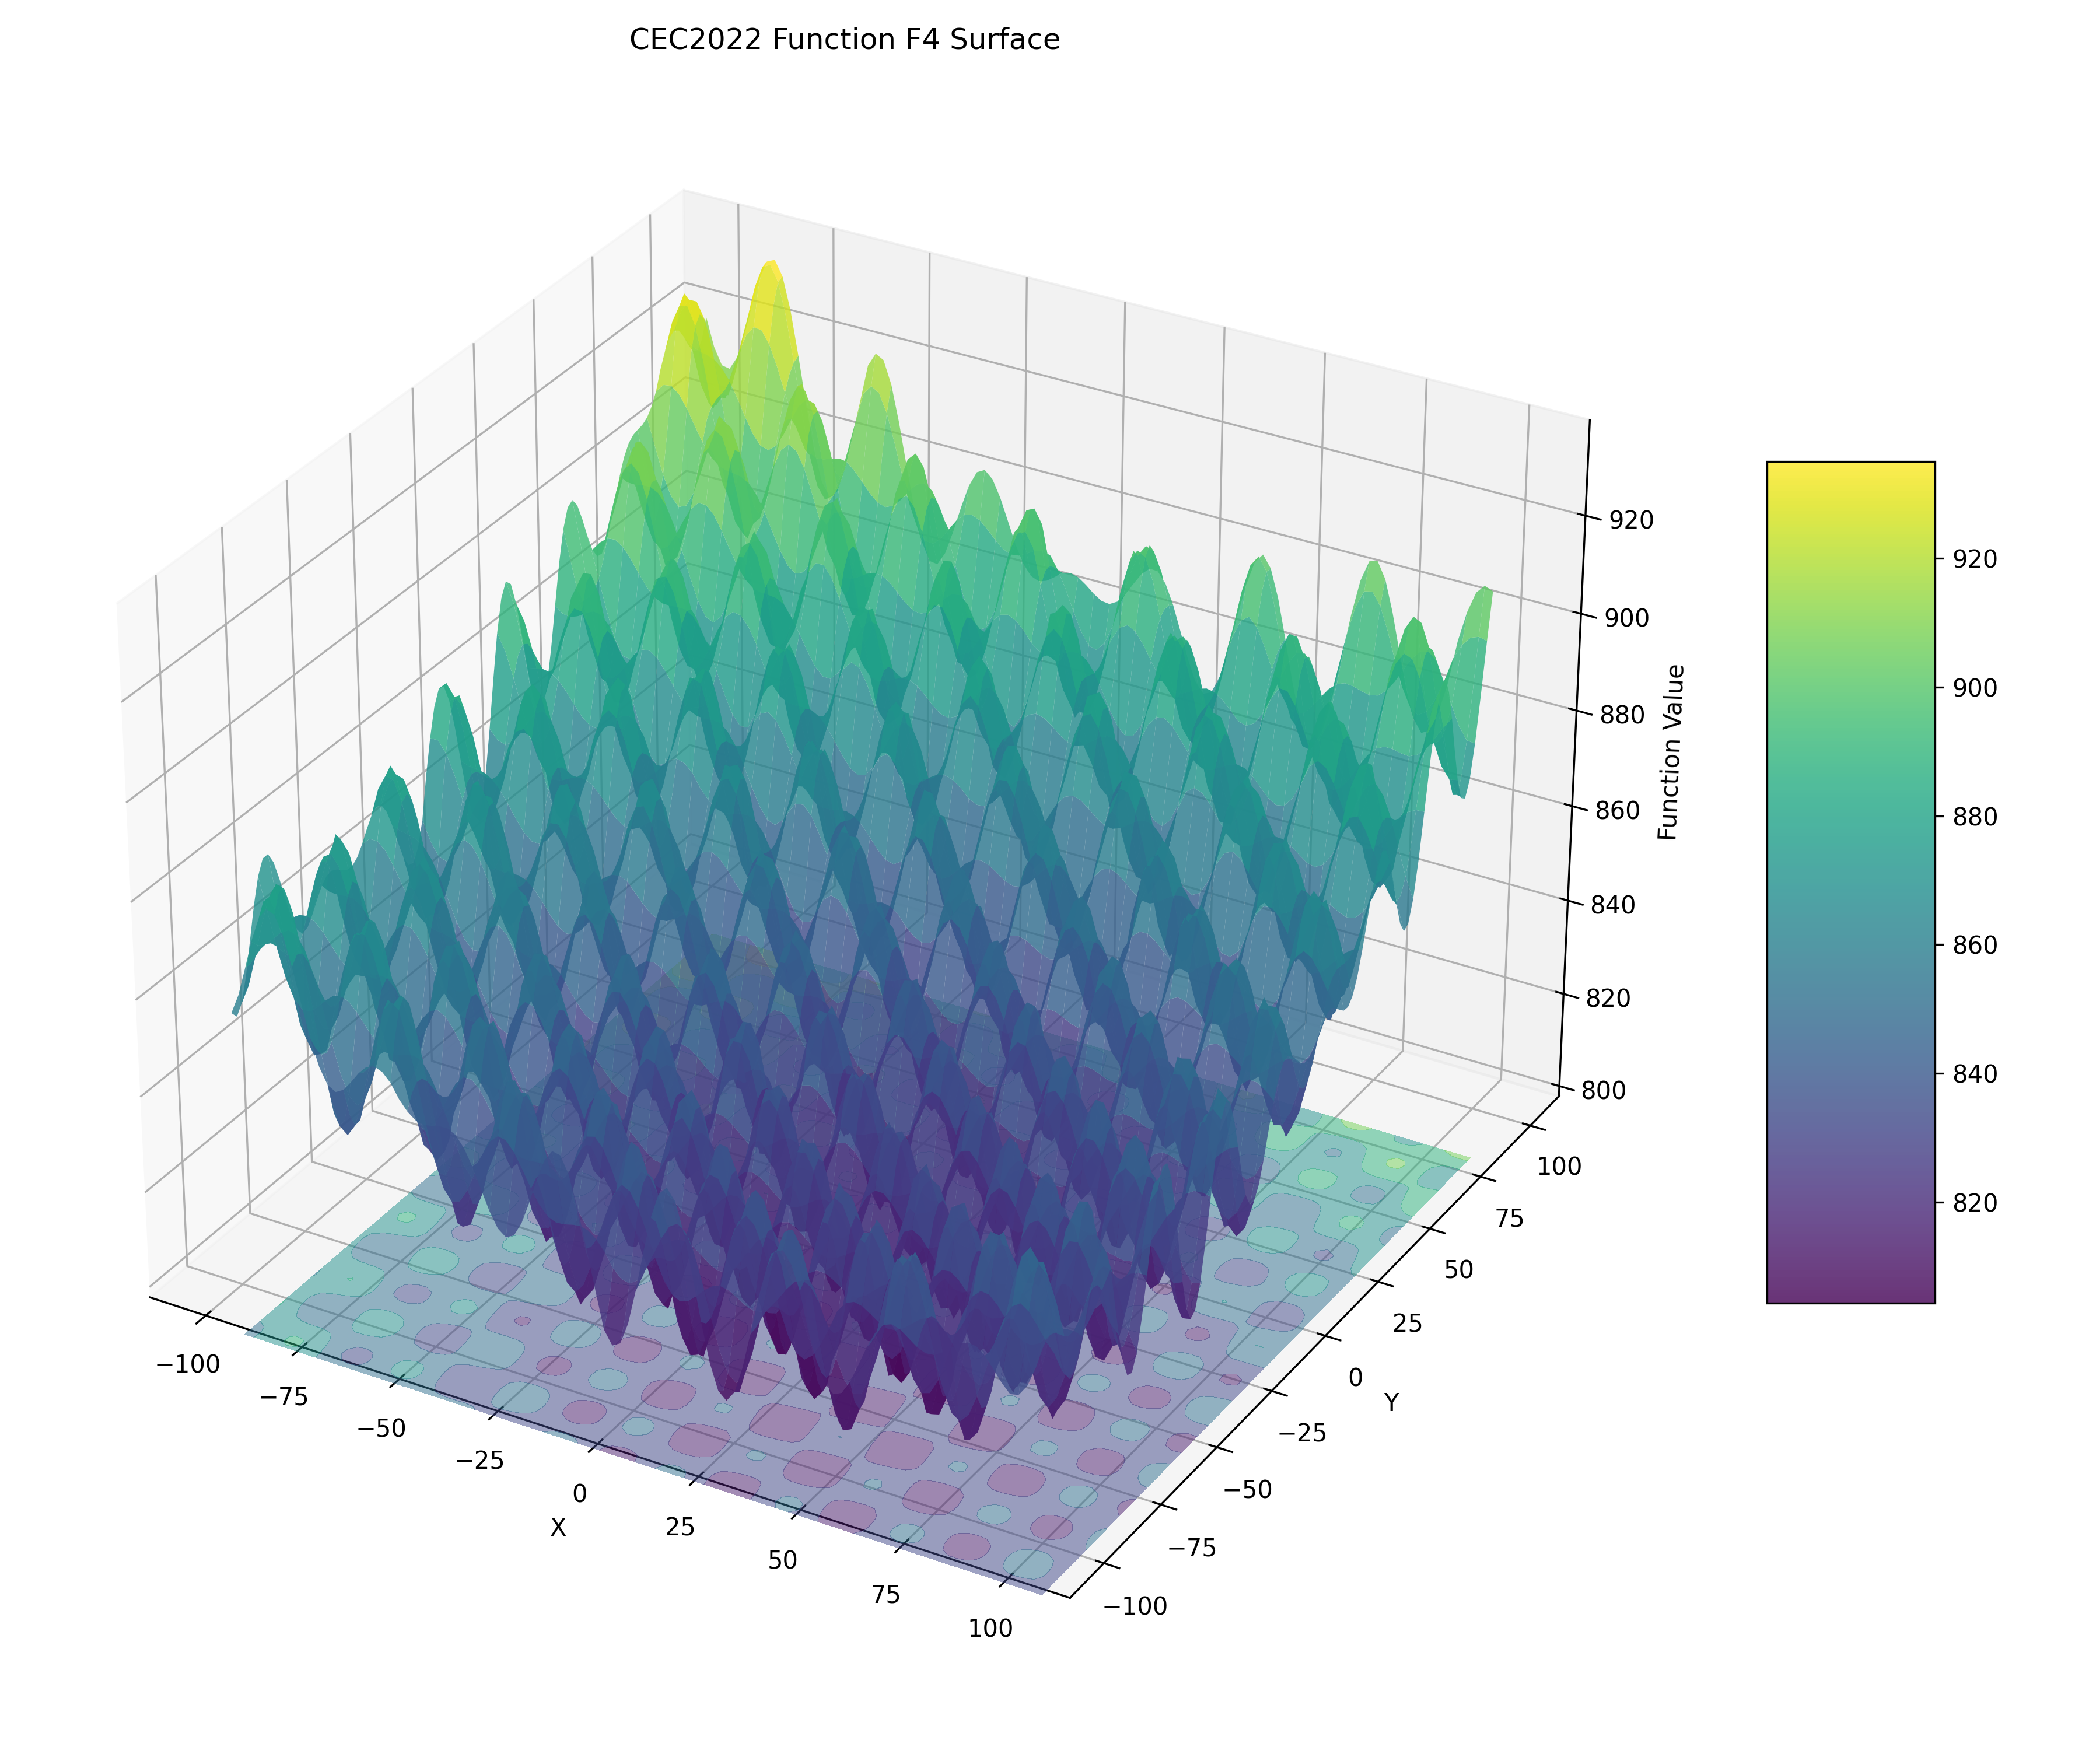
\includegraphics[width=\textwidth]{../plots/cec_bench/function_surface_f4.png}
            \caption*{F4}
        \end{subfigure}
        \hfill
        \begin{subfigure}[b]{0.19\textwidth}
            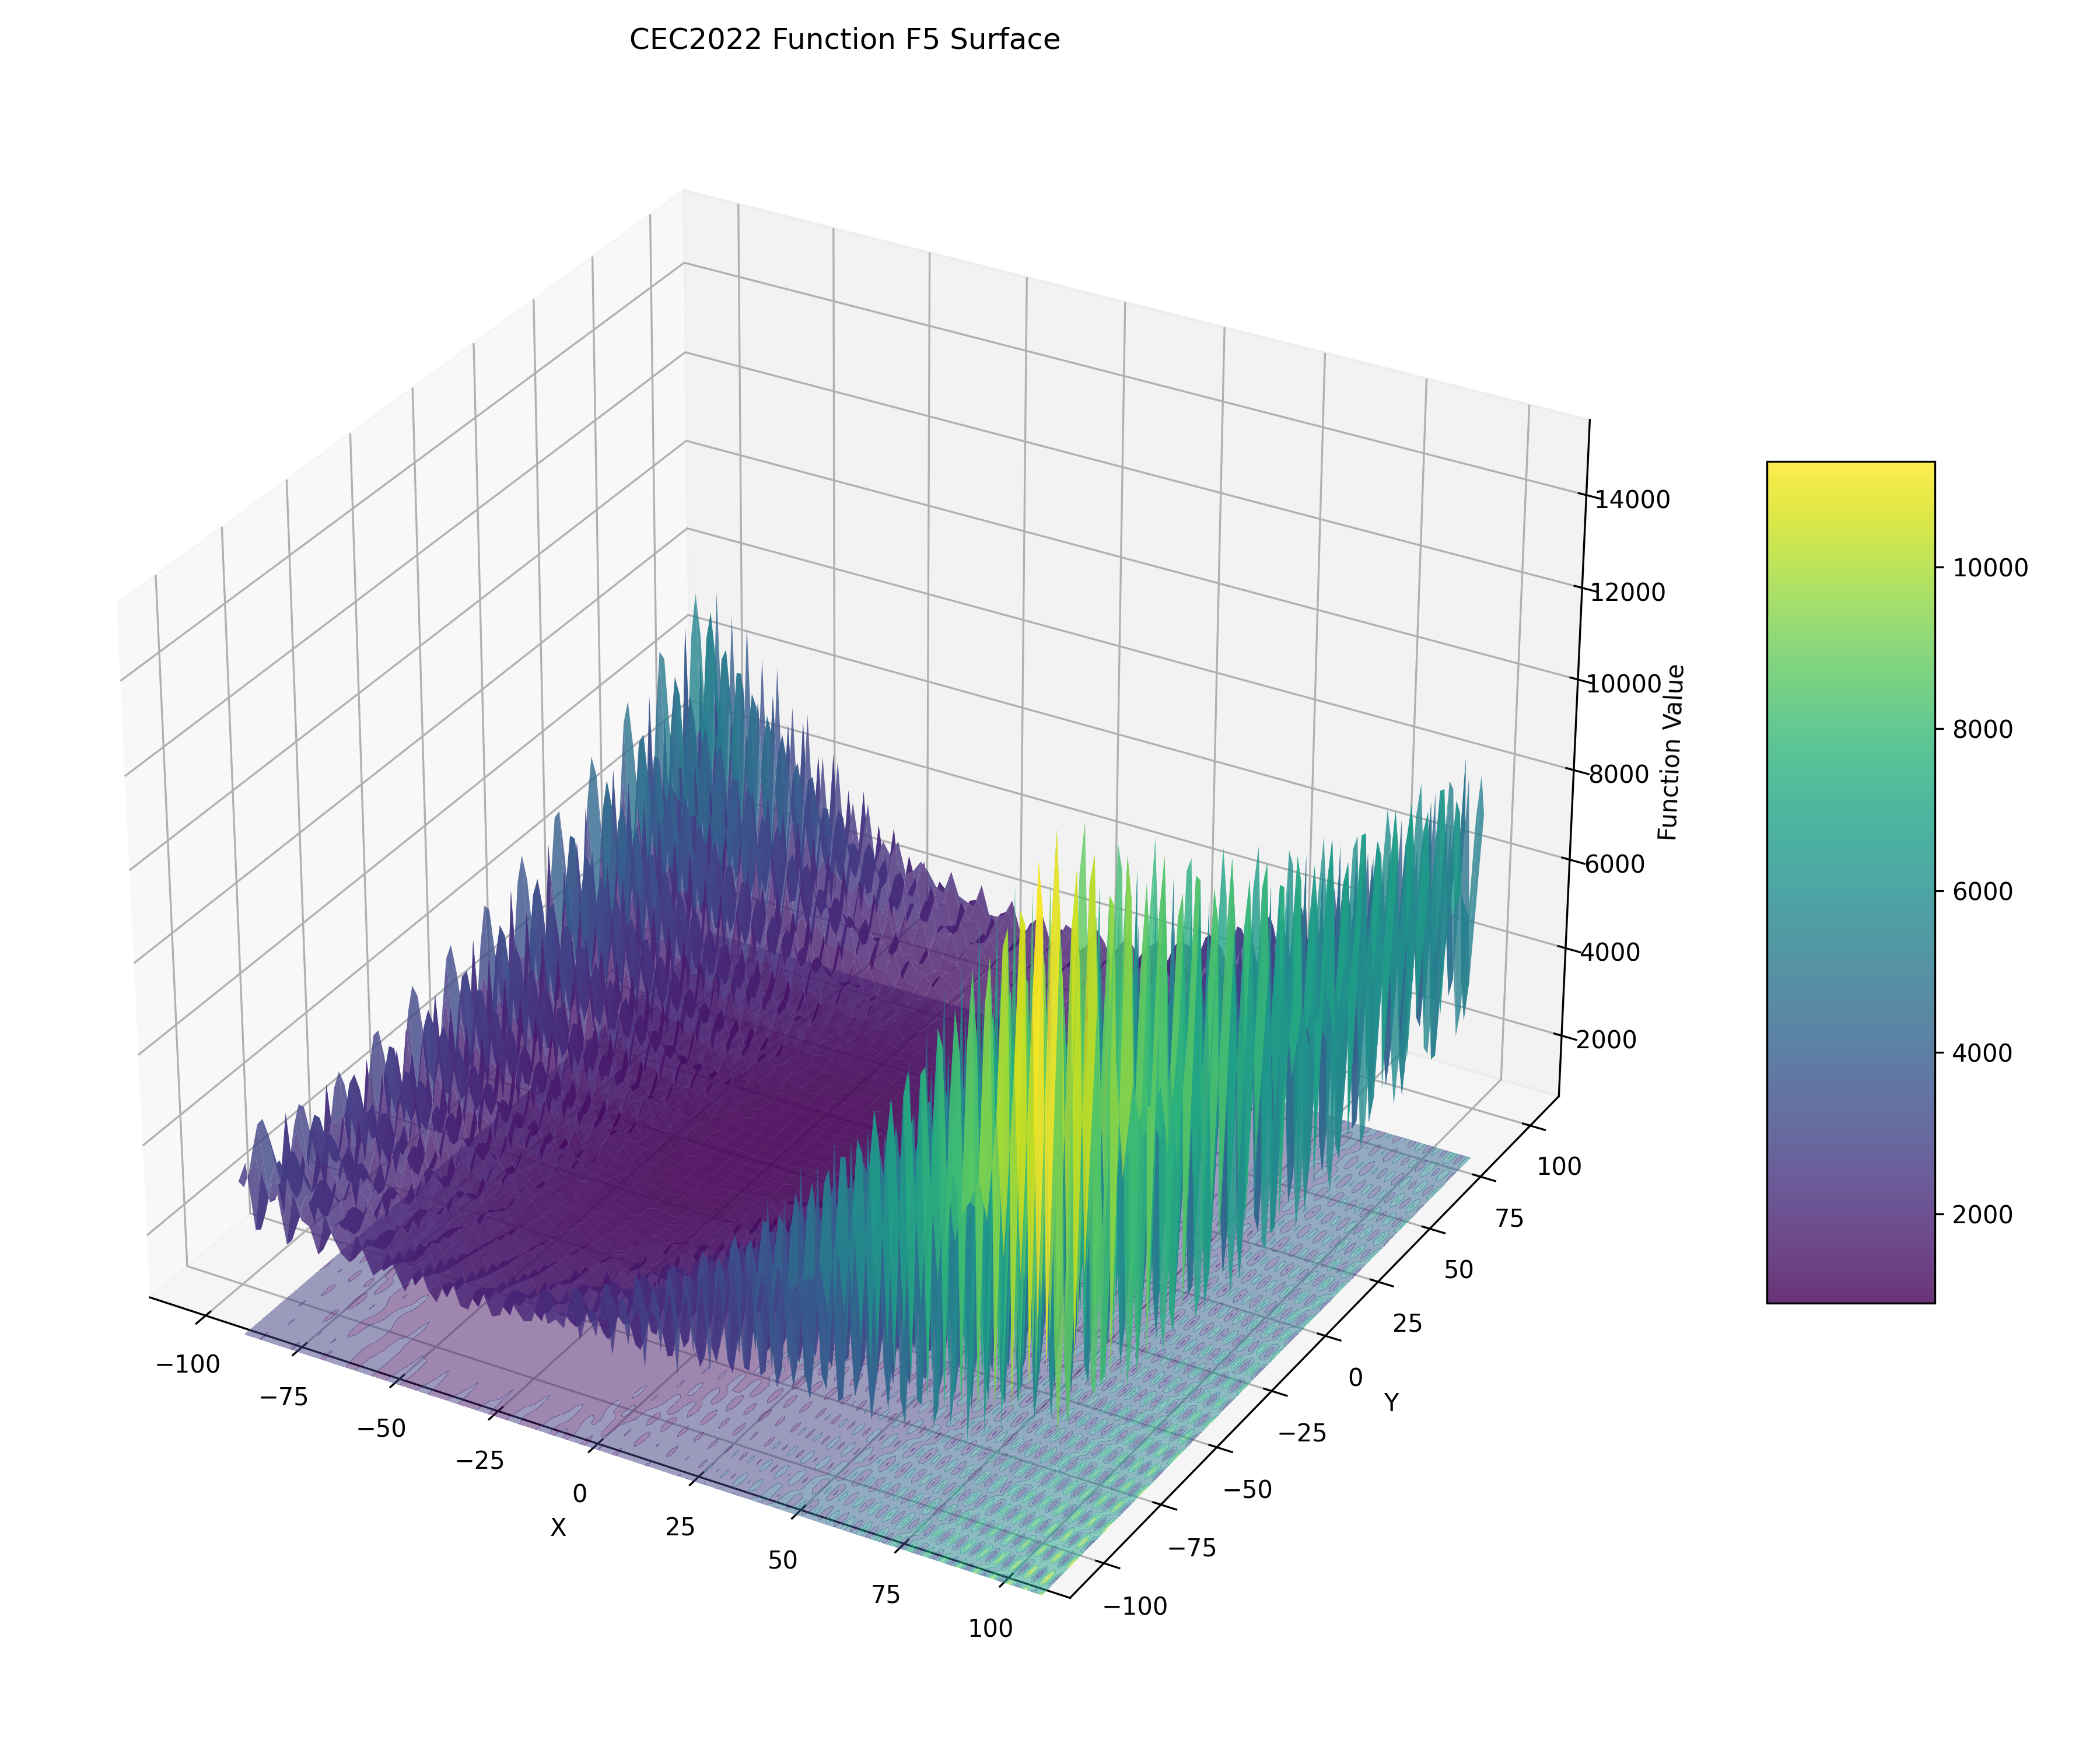
\includegraphics[width=\textwidth]{../plots/cec_bench/function_surface_f5.png}
            \caption*{F5}
        \end{subfigure}
        \vspace{-1ex}
        \caption*{\scriptsize Function surfaces for CEC benchmark functions}
    \end{figure}
\end{frame}

% % % % ------------------------ APSO Optimization ------------------------
\begin{frame}{APSO Optimization Visulization}
    \centering
    \begin{figure}
        \centering
        % First row
        \begin{subfigure}[b]{0.20\textwidth}
            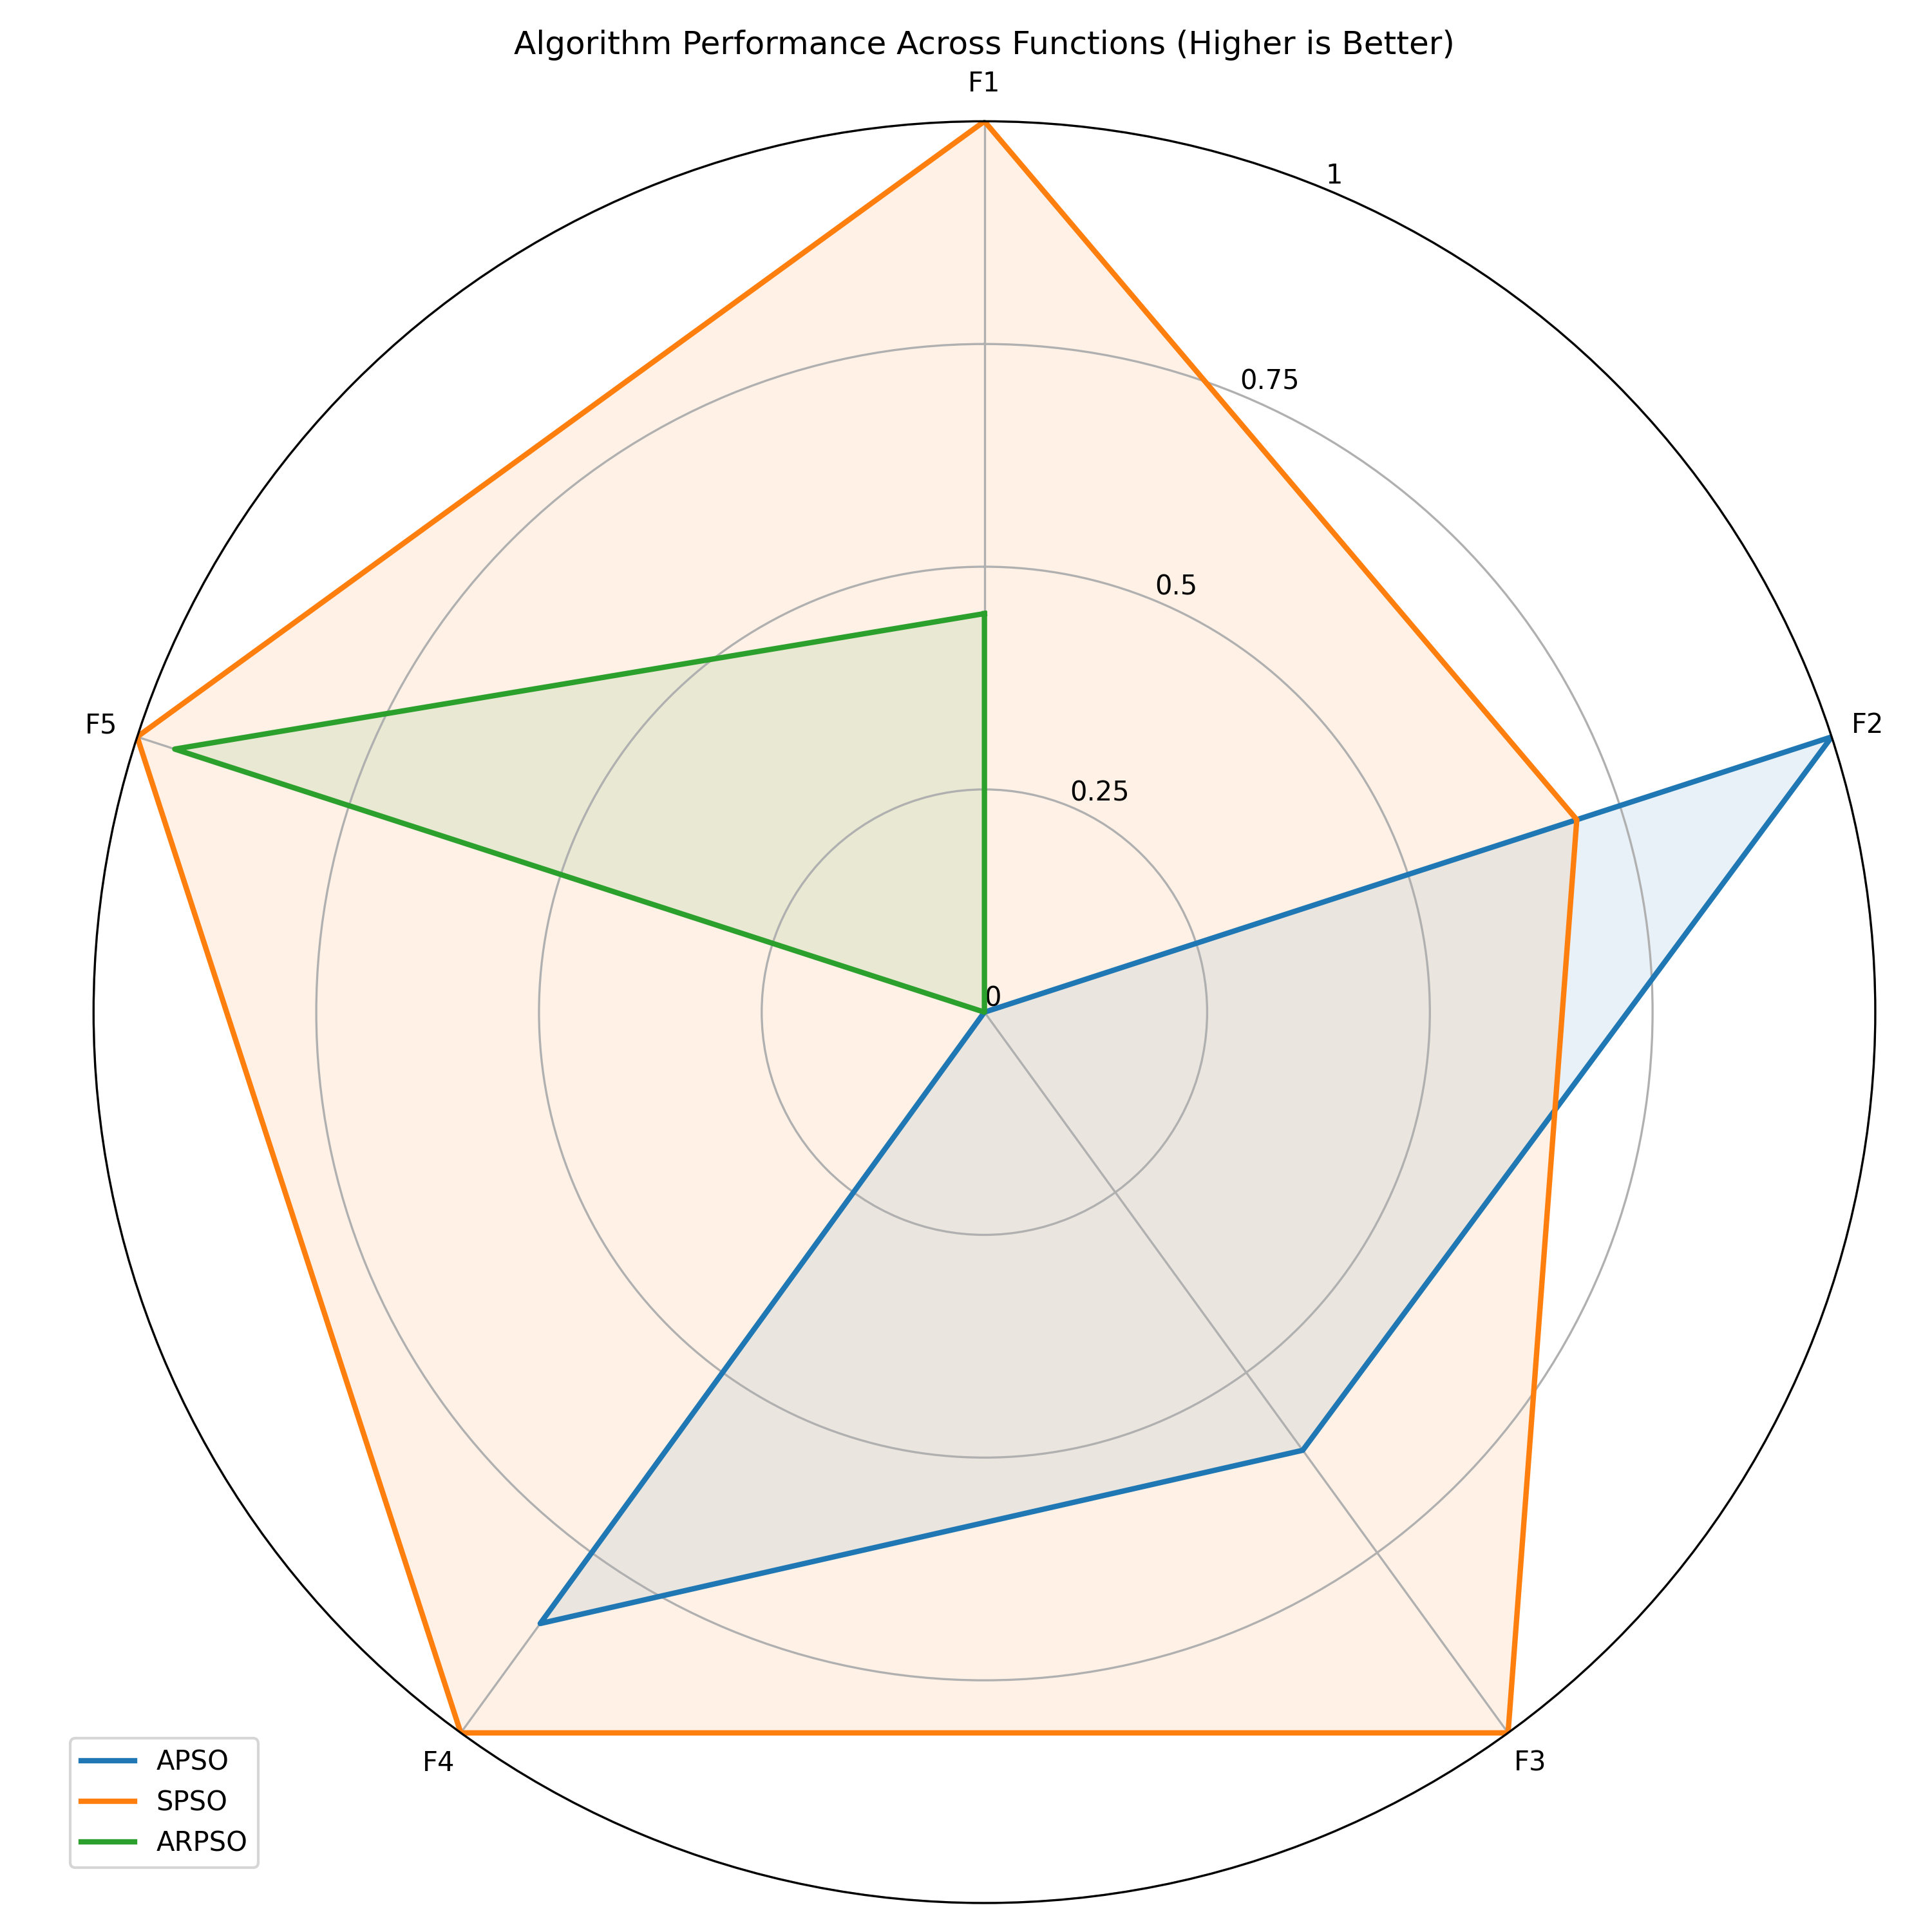
\includegraphics[width=\textwidth]{../plots/cec_bench/radar_chart.png}
            \caption*{PSO's Performance across functions}
        \end{subfigure}
        % \hfill
        \begin{subfigure}[b]{0.34\textwidth}
            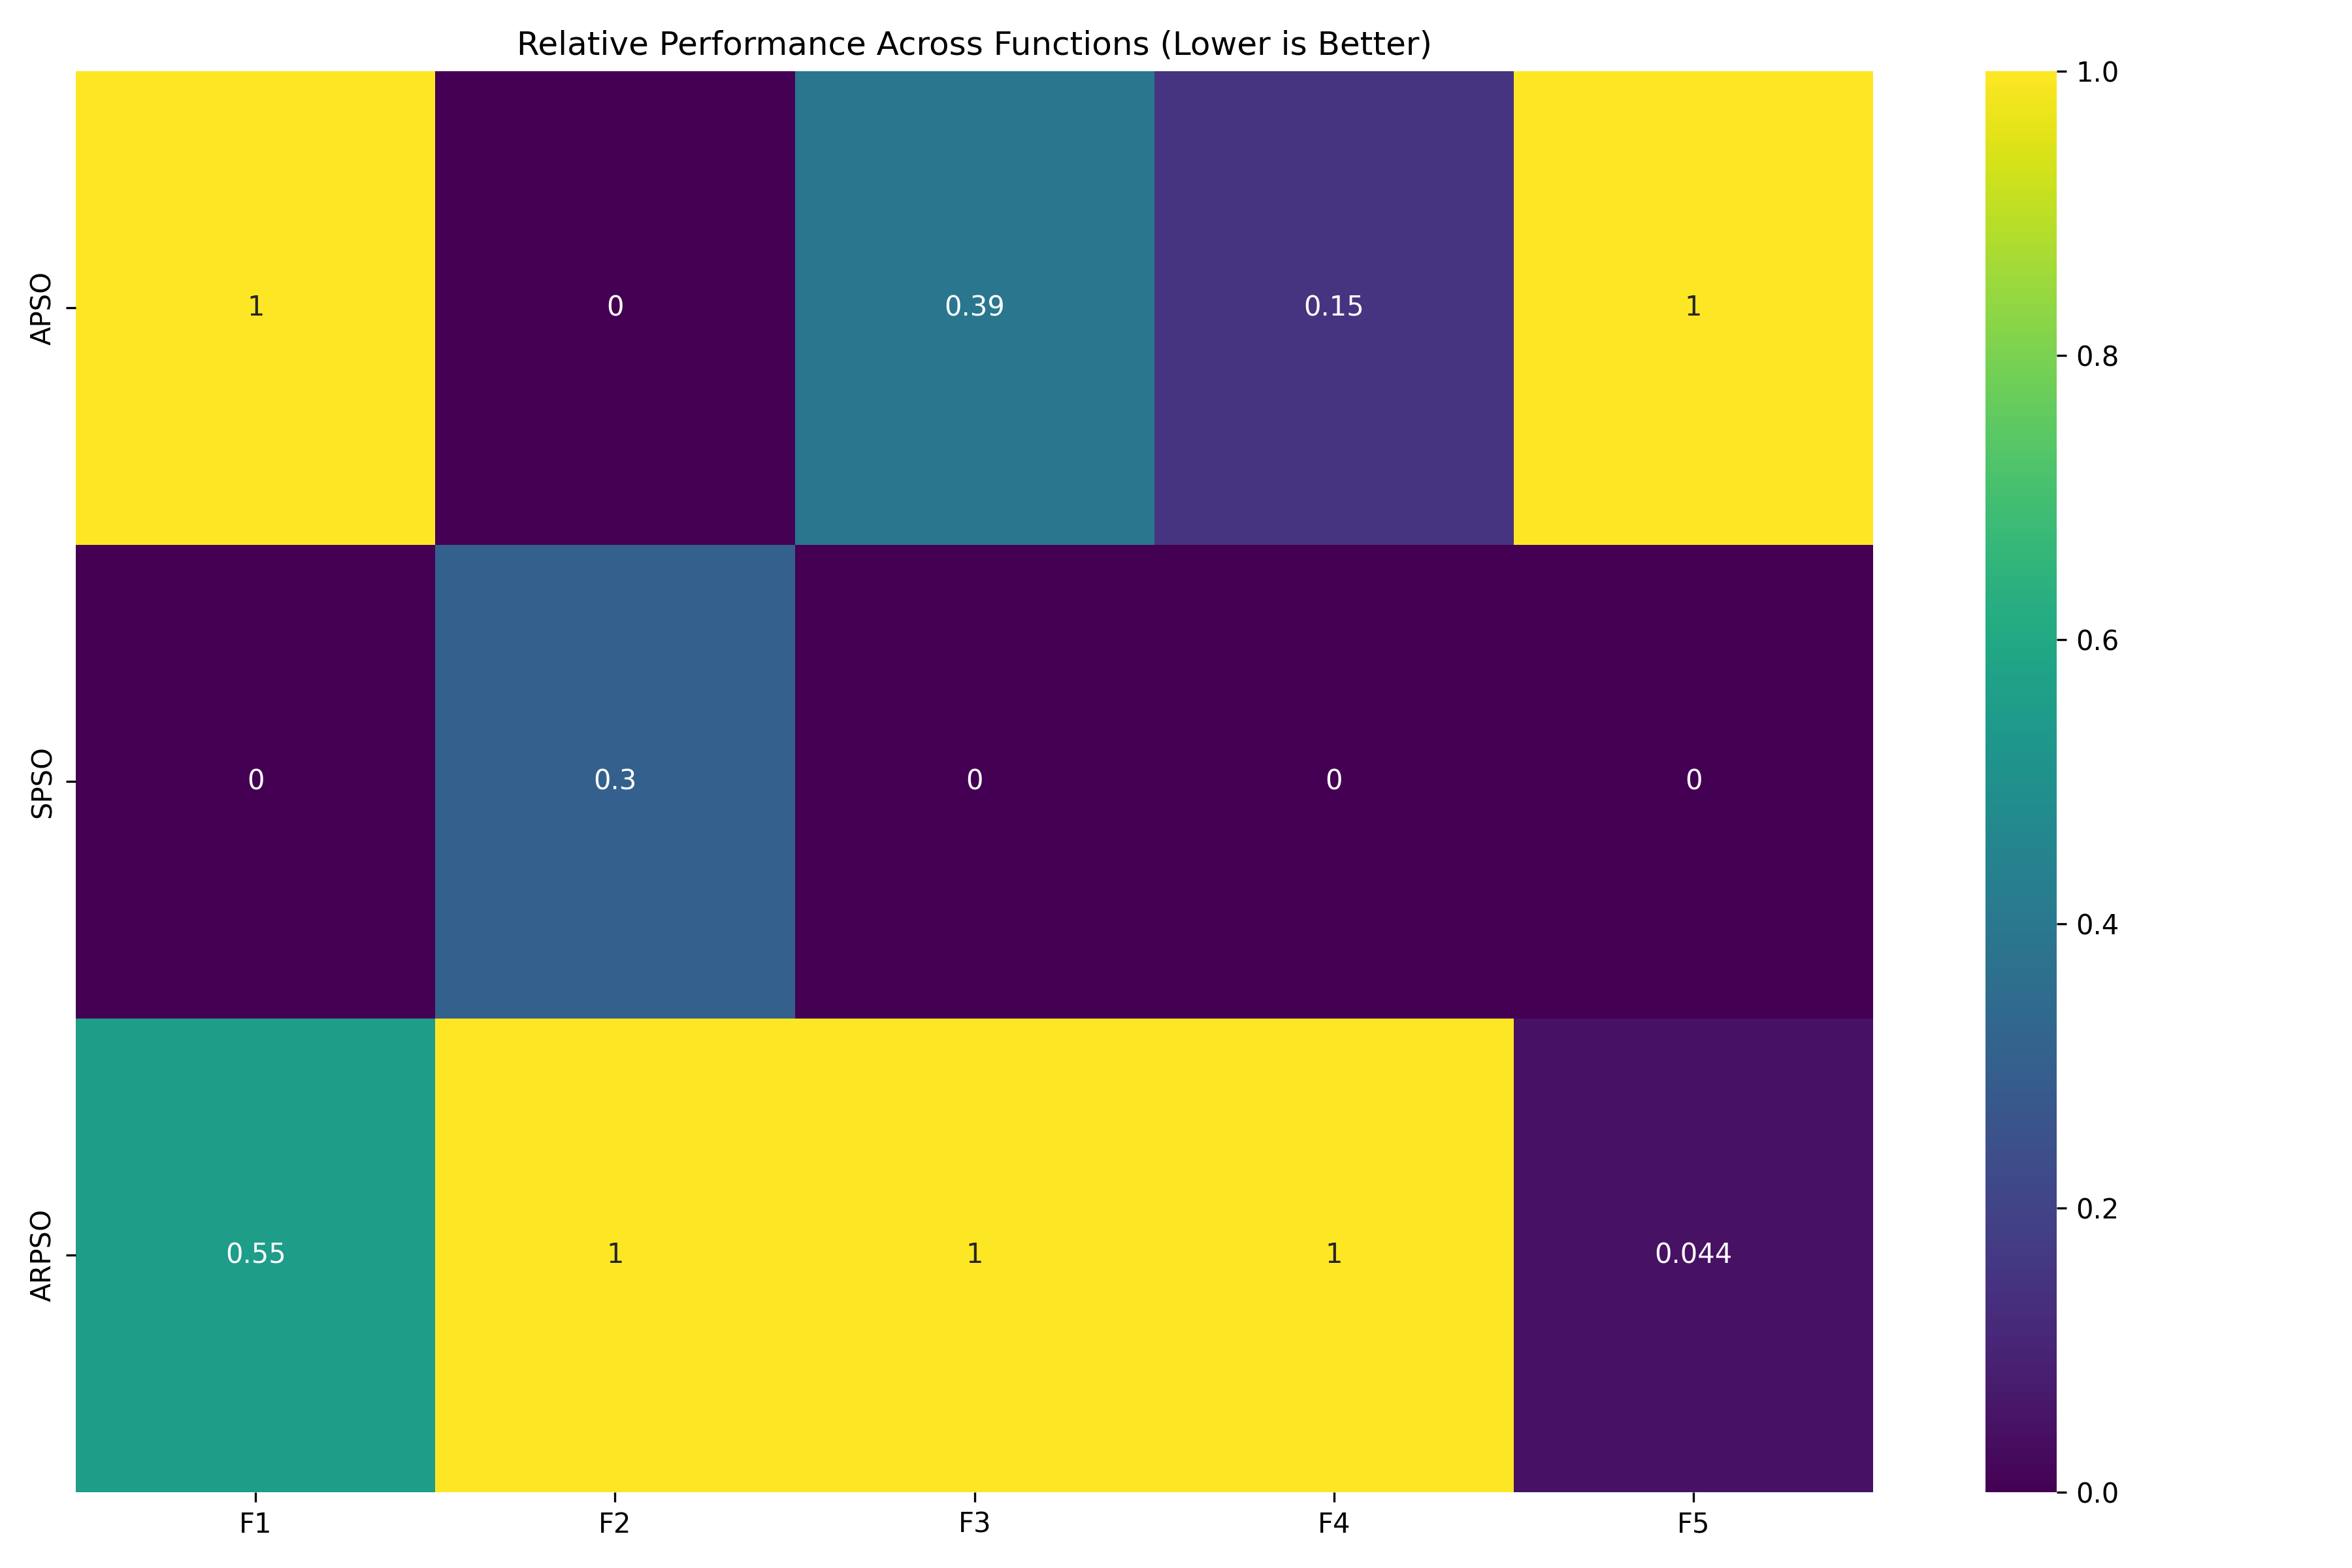
\includegraphics[width=\textwidth]{../plots/cec_bench/performance_heatmap.png}
            \caption*{Relative Performance Across function}
        \end{subfigure}
        \vspace{-1ex}
        \caption*{\scriptsize Performance Matrix}
    \end{figure}
    
    \vspace{-1ex}
    {\scriptsize For 2D,3D visualization of APSO optimization on Functions, visit: 
    \href{https://github.com/pingu-73/vigilant-spork/tree/main/plots/cec_bench/gifs}{\textcolor{blue}{@pingu-73/vigilant-spork/../gifs}}}
\end{frame}

\begin{frame}
    \centering
    \begin{figure}
        \centering
        % First row
        \begin{subfigure}[b]{0.19\textwidth}
            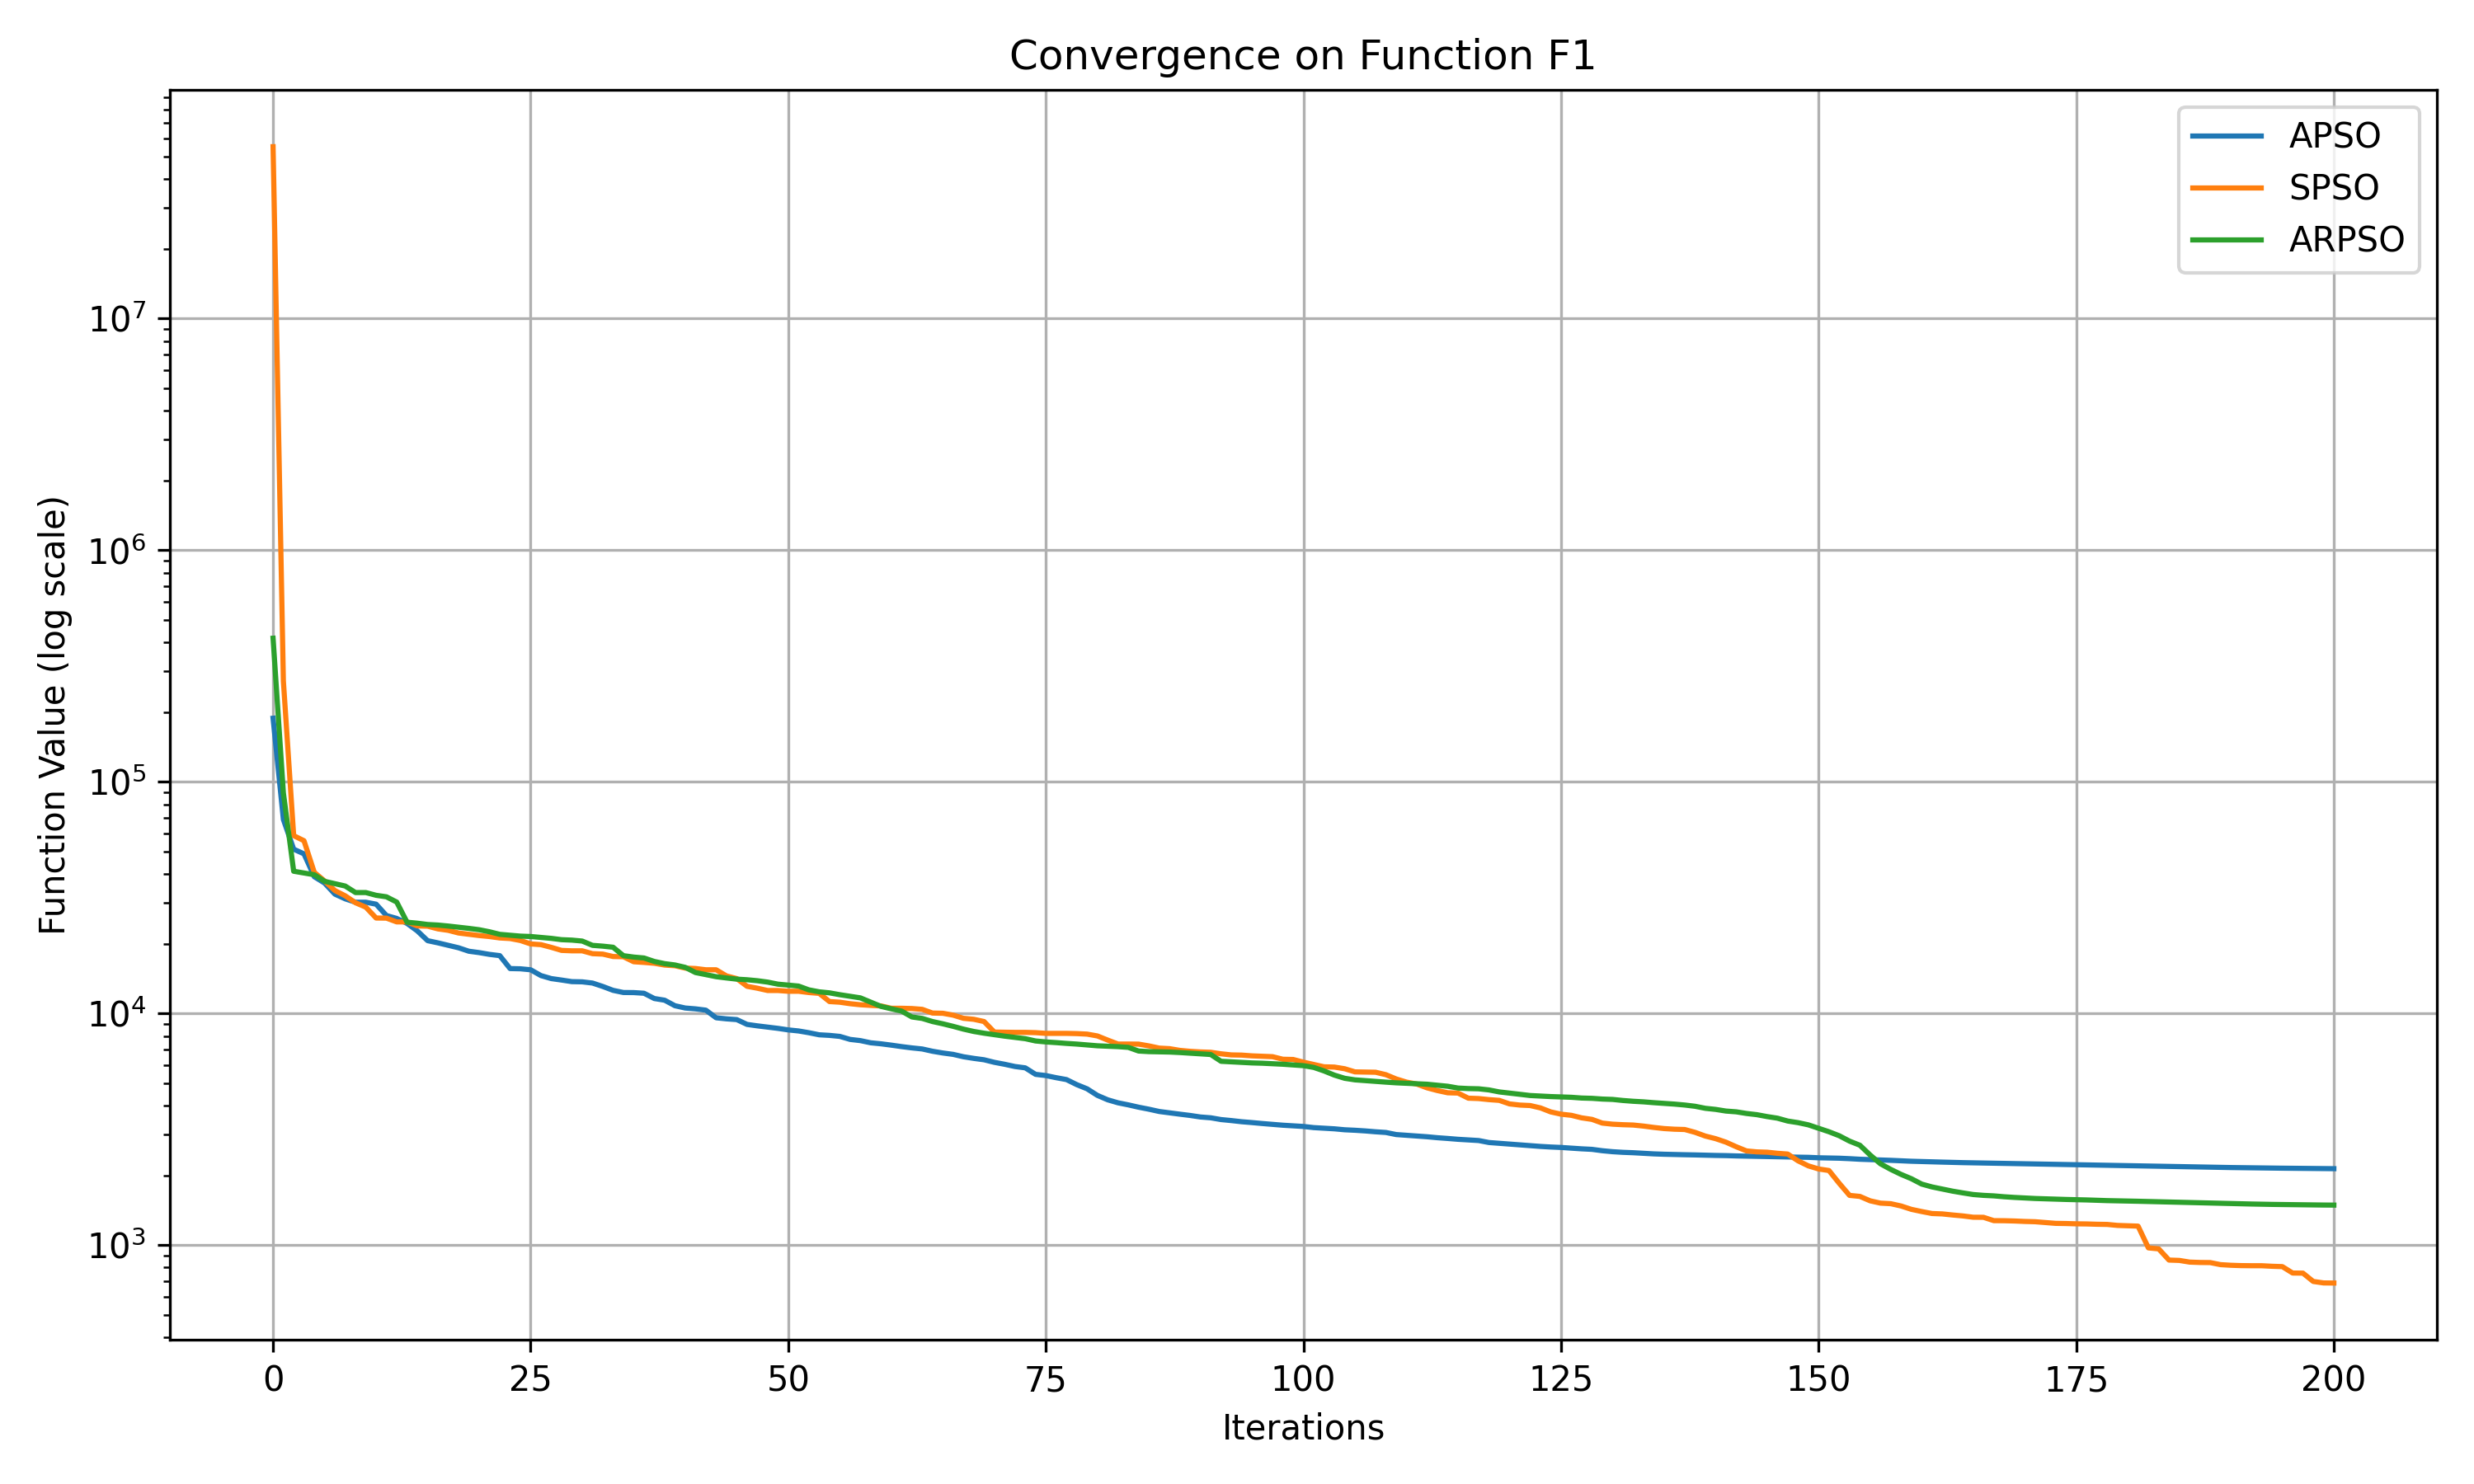
\includegraphics[width=\textwidth]{../plots/cec_bench/cec_convergence_f1.png}
            \caption*{F1 convergence}
        \end{subfigure}
        \hfill
        \begin{subfigure}[b]{0.19\textwidth}
            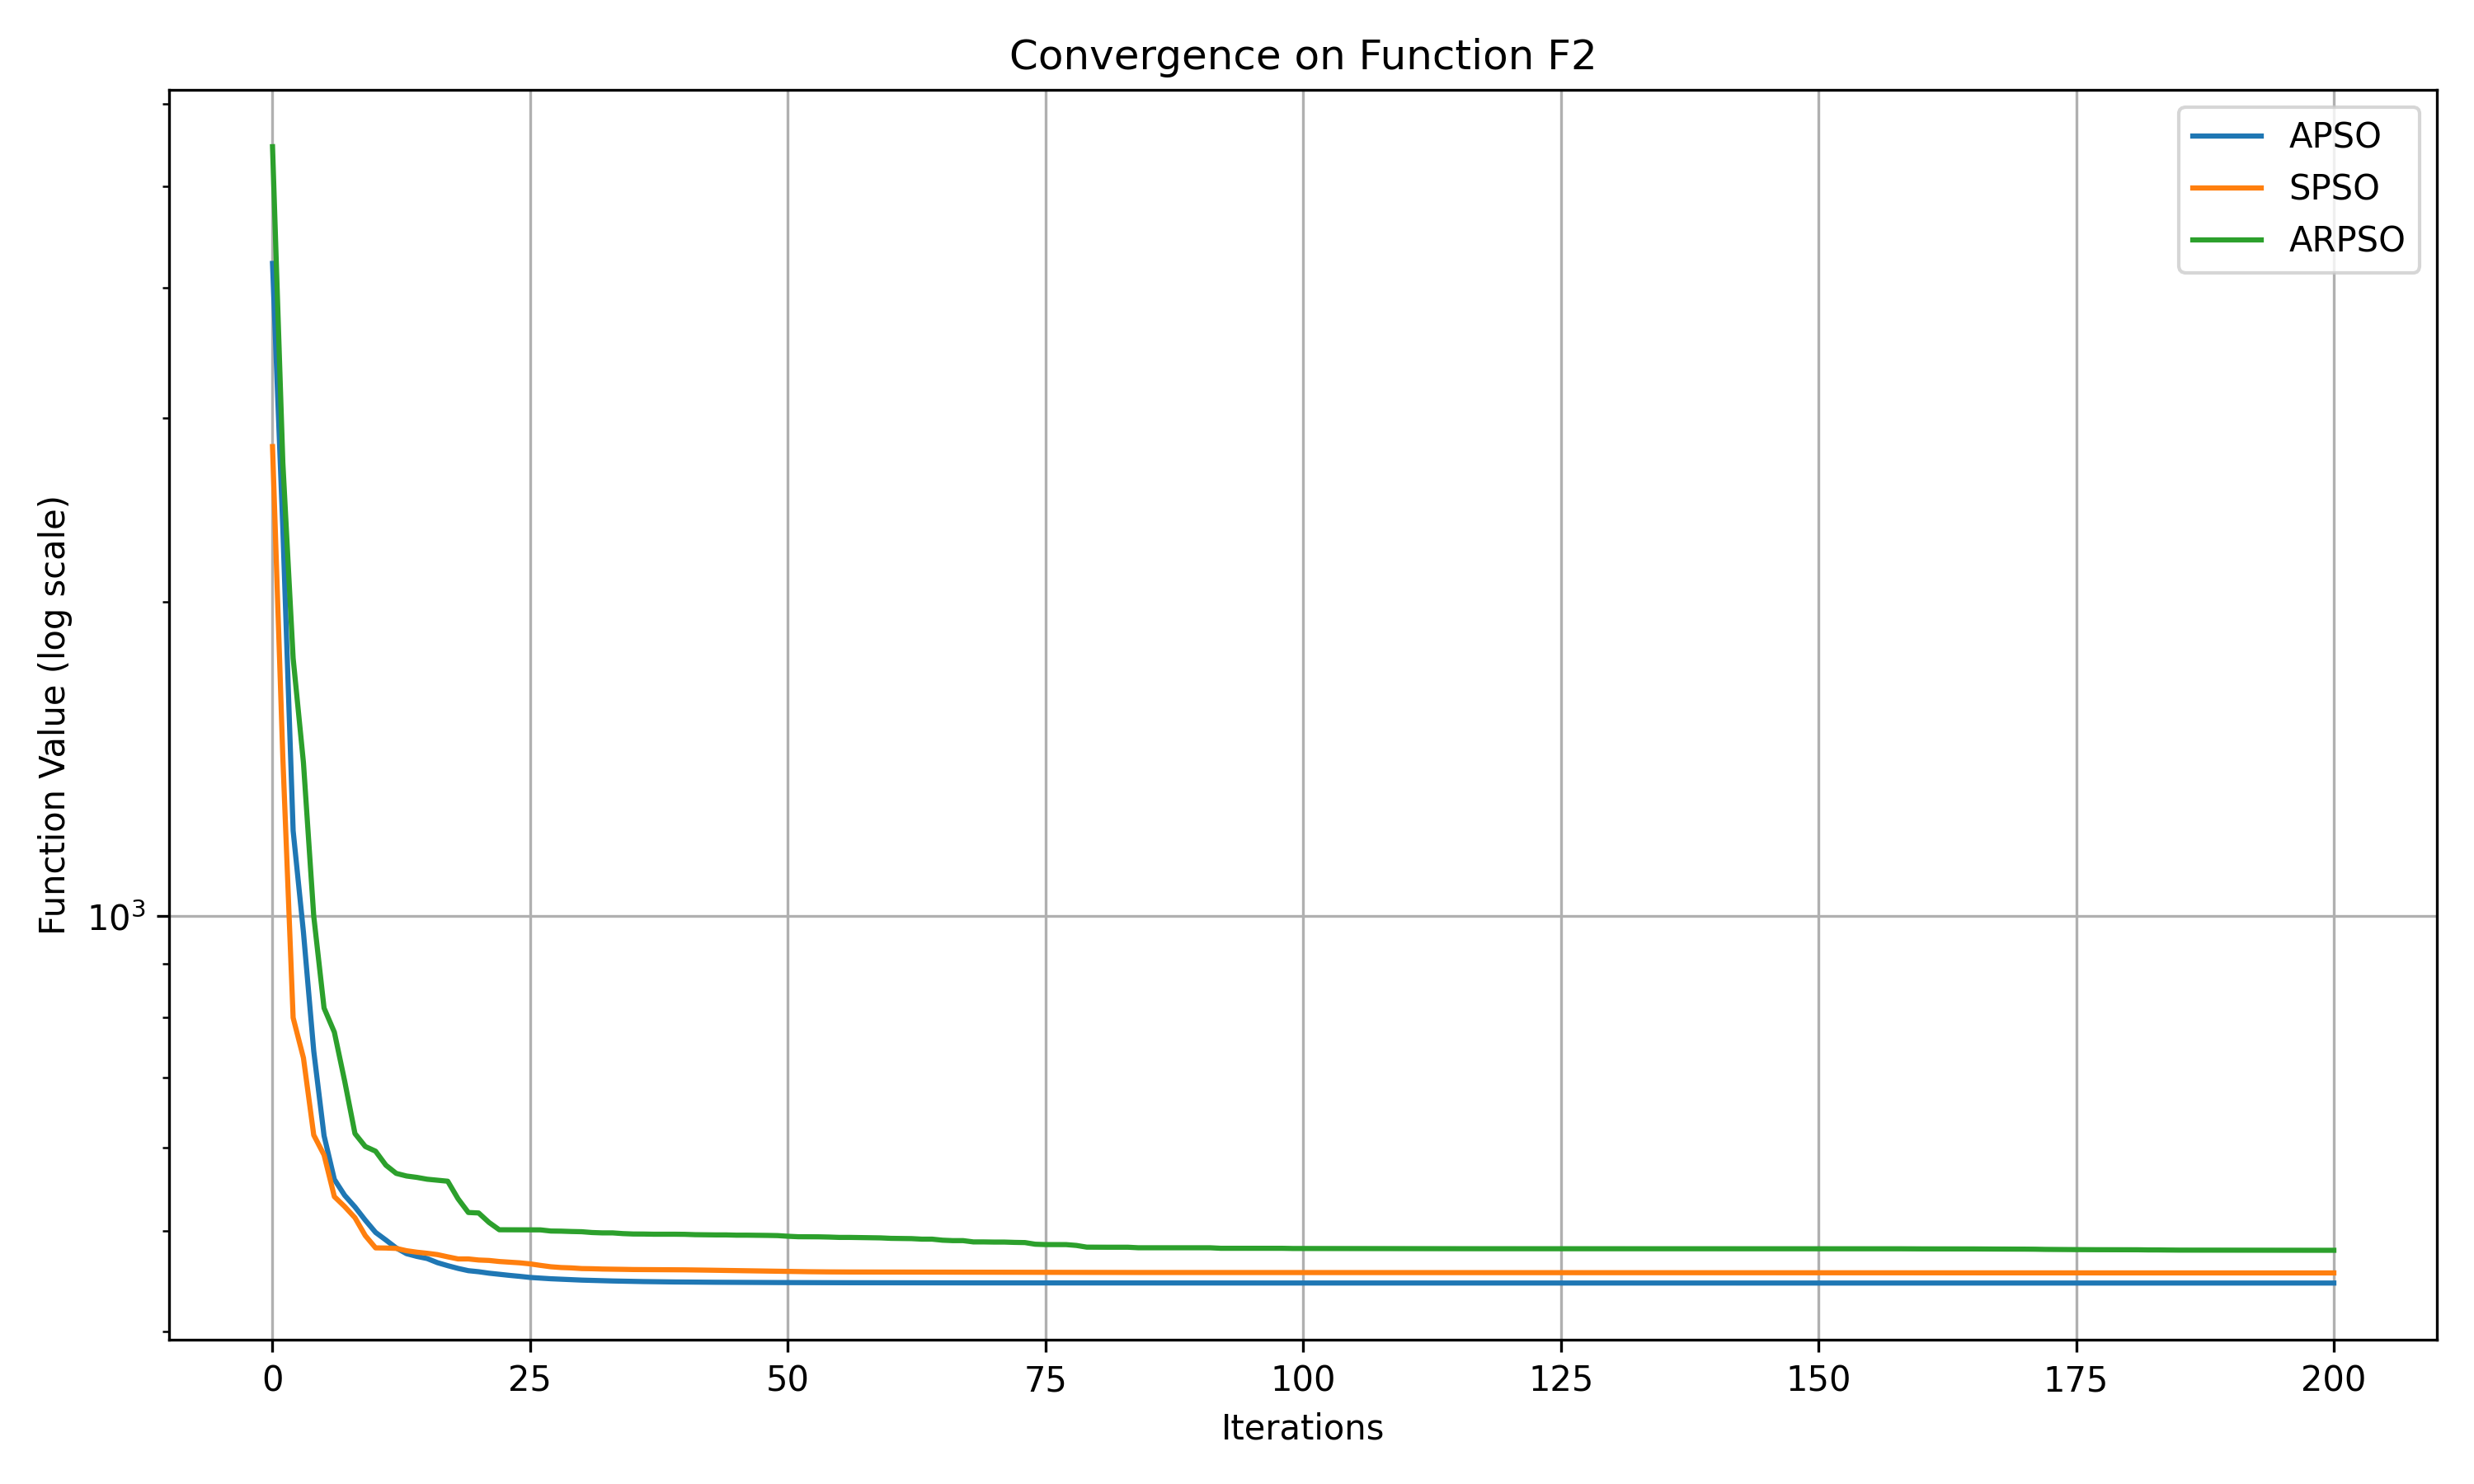
\includegraphics[width=\textwidth]{../plots/cec_bench/cec_convergence_f2.png}
            \caption*{F2 convergence}
        \end{subfigure}
        \hfill
        \begin{subfigure}[b]{0.19\textwidth}
            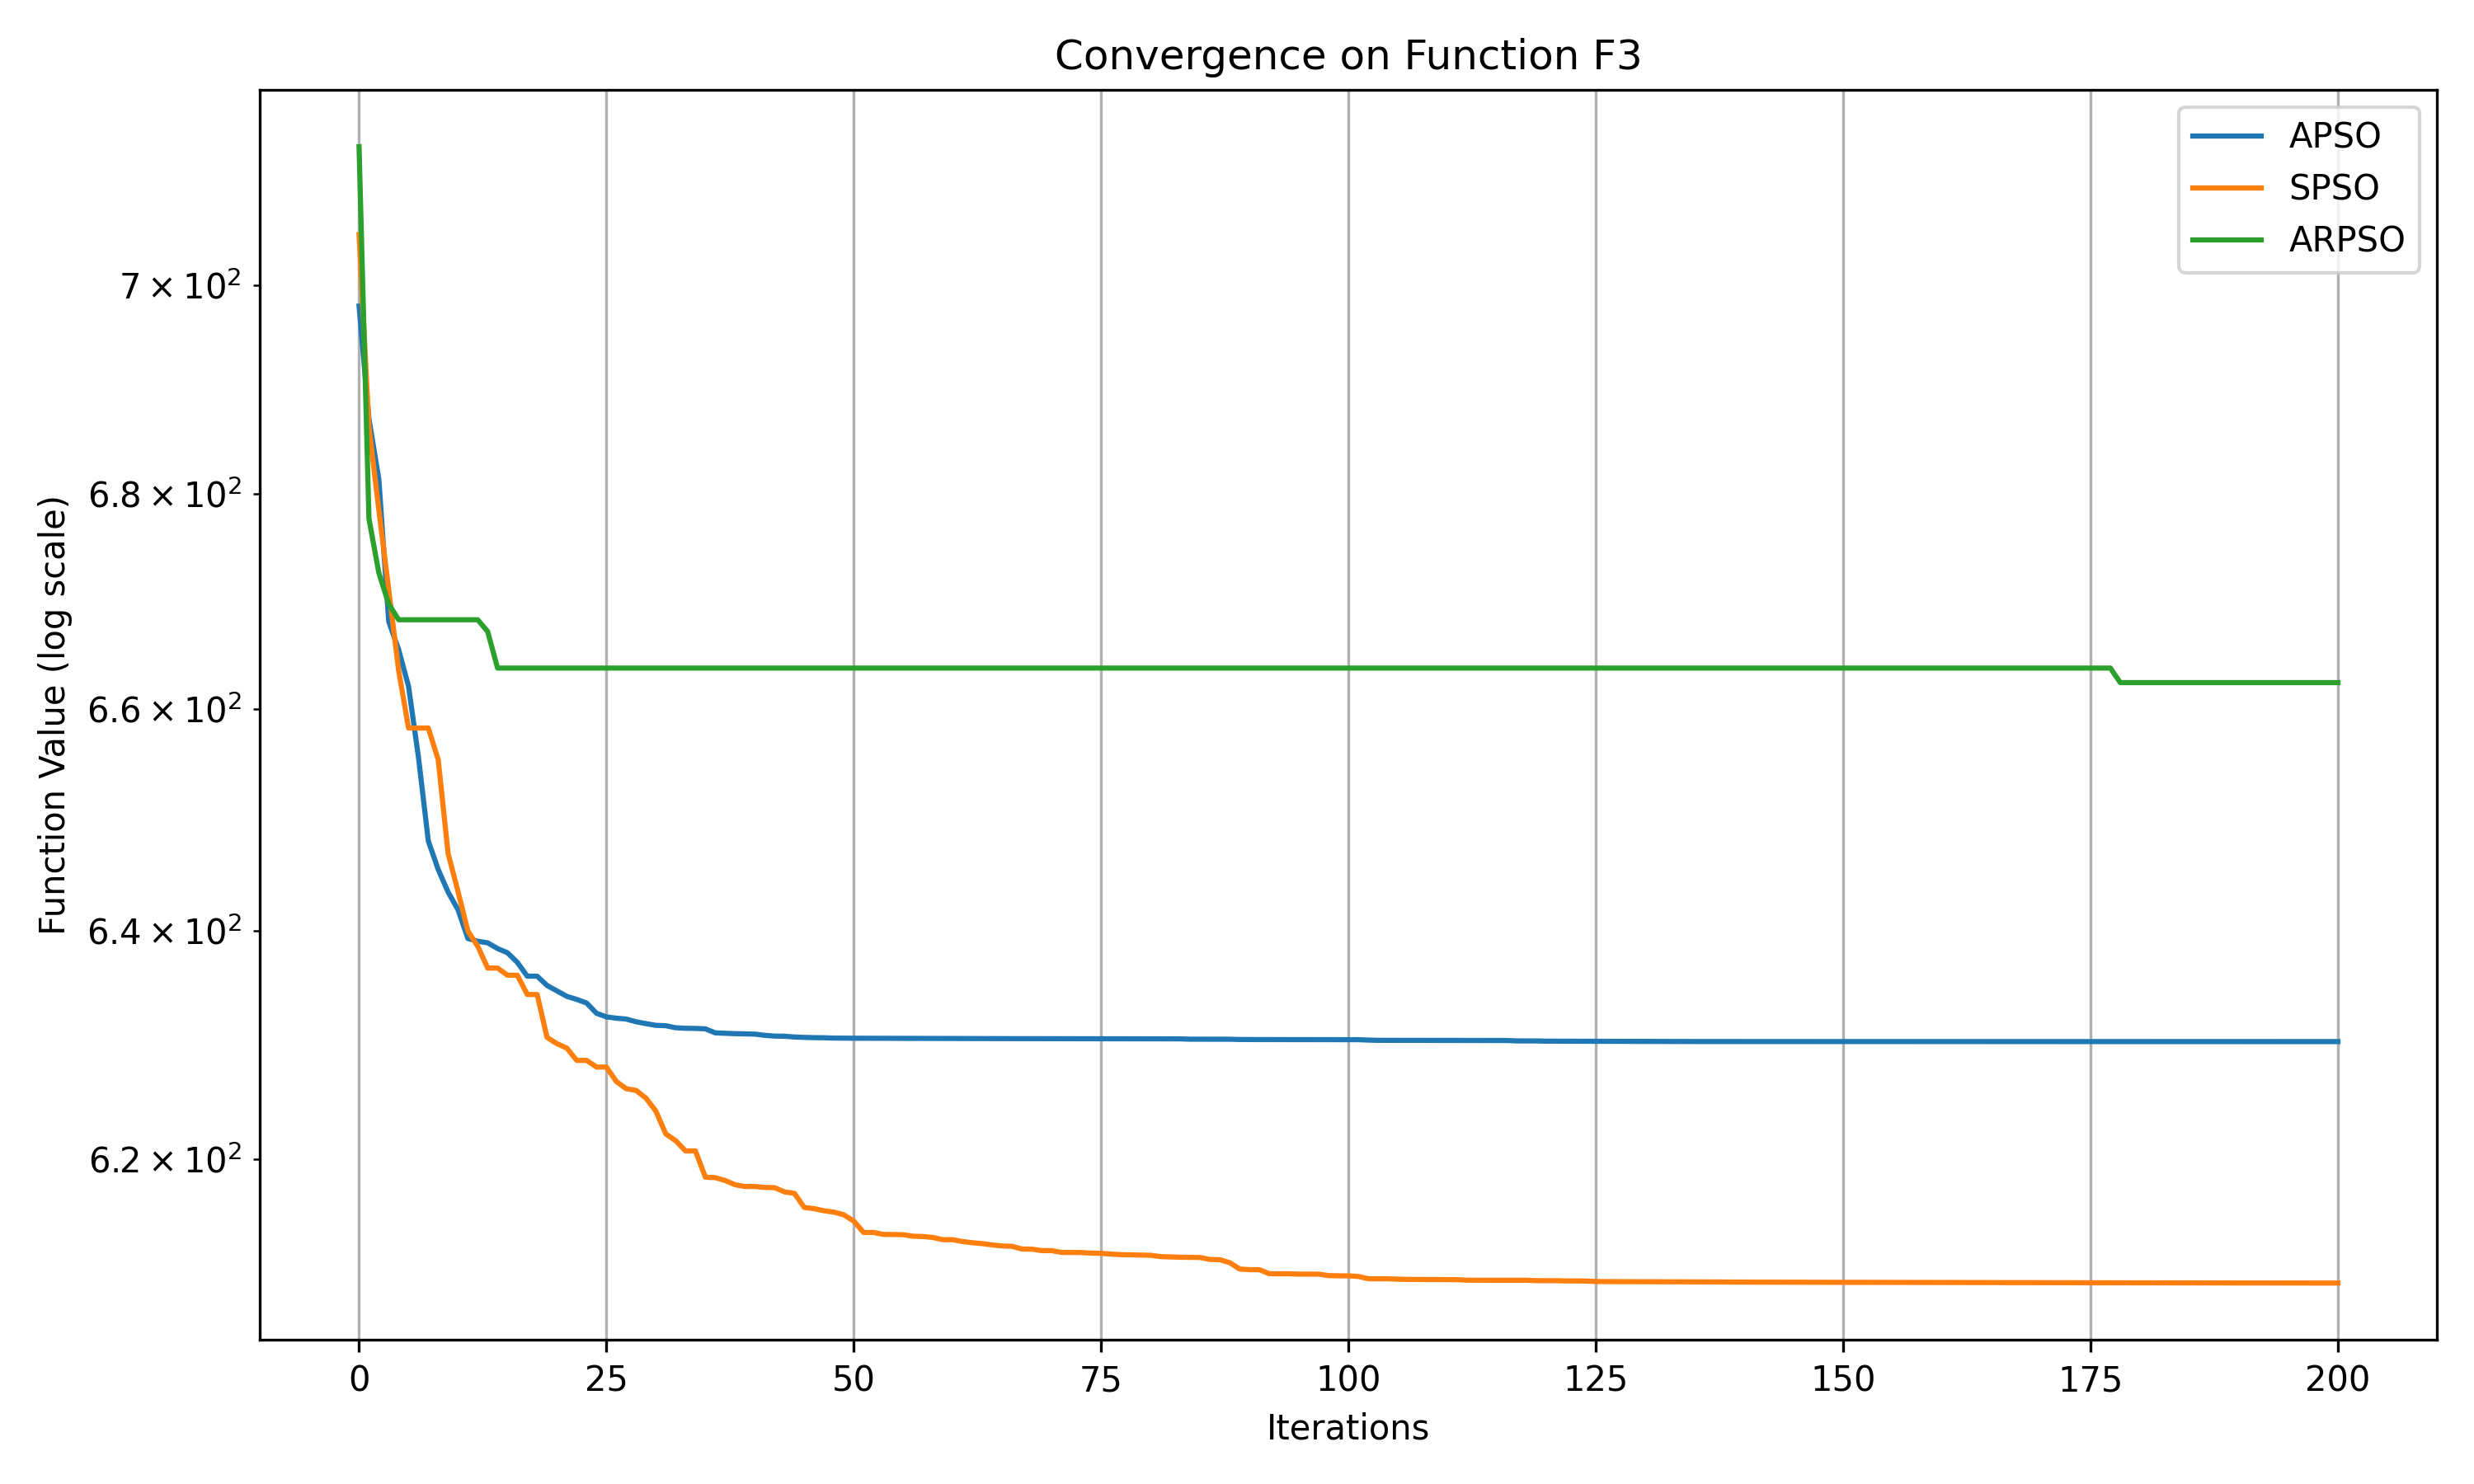
\includegraphics[width=\textwidth]{../plots/cec_bench/cec_convergence_f3.png}
            \caption*{F3 convergence}
        \end{subfigure}
        \hfill
        \begin{subfigure}[b]{0.19\textwidth}
            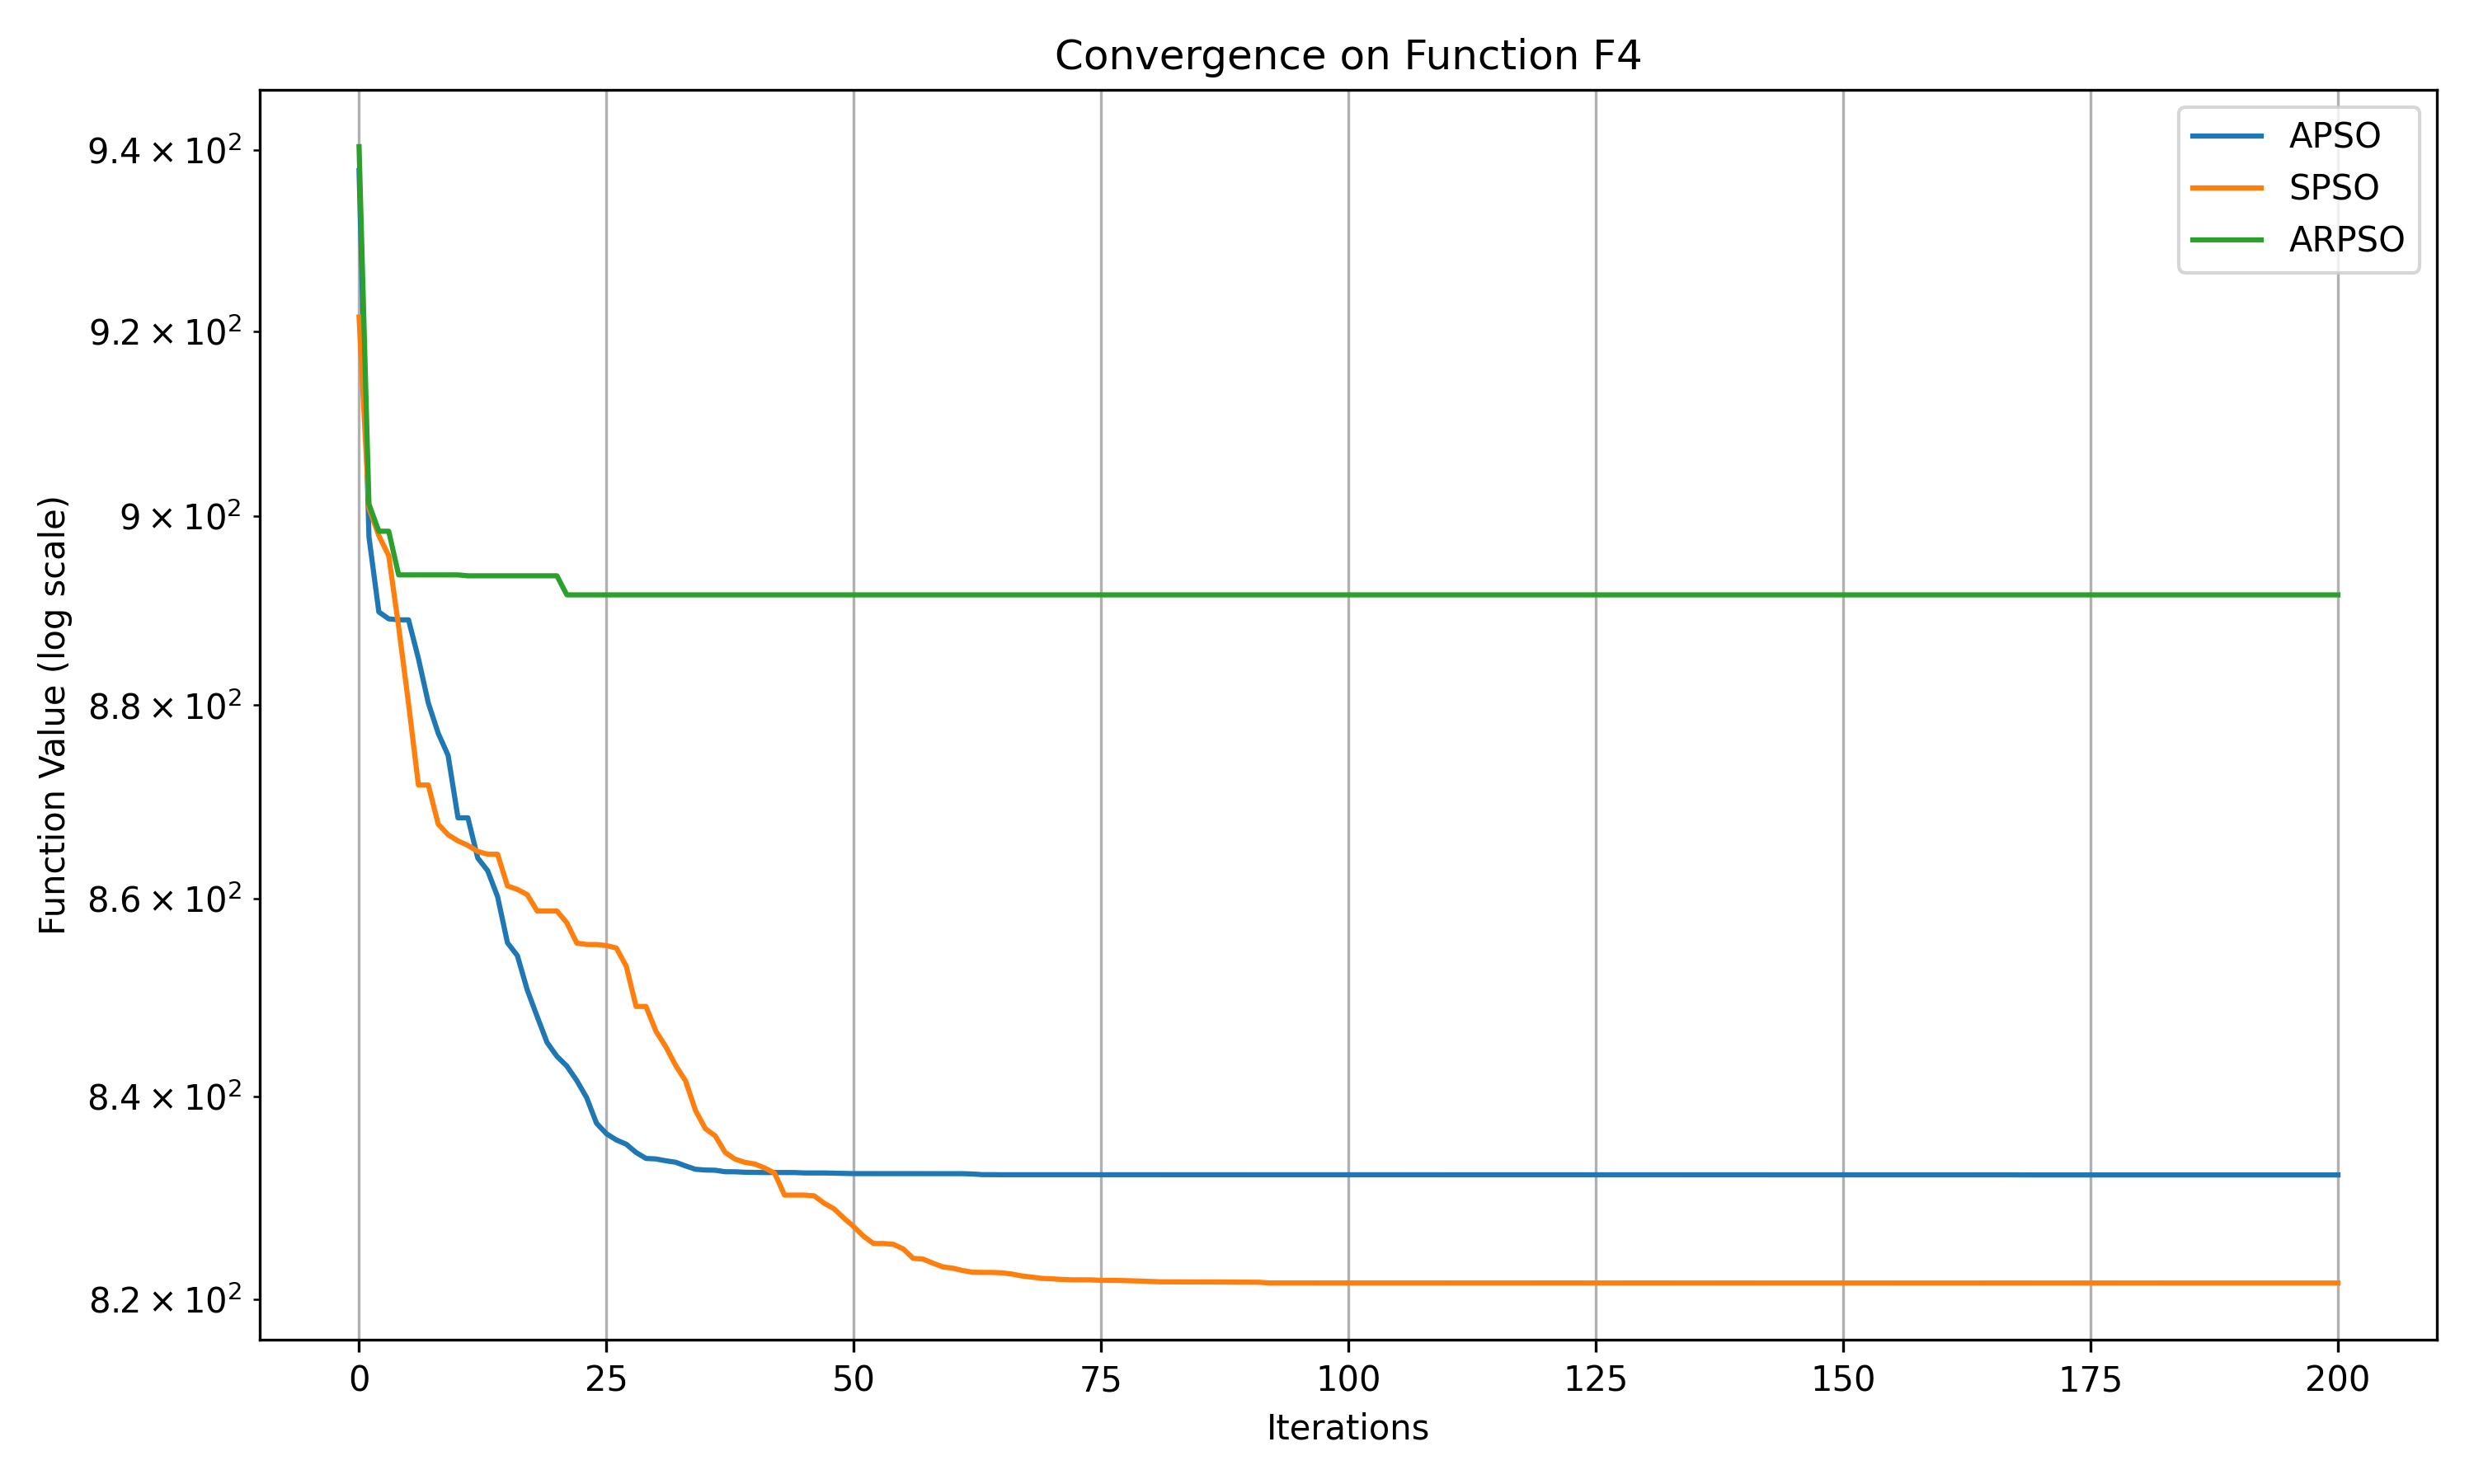
\includegraphics[width=\textwidth]{../plots/cec_bench/cec_convergence_f4.png}
            \caption*{F4 convergence}
        \end{subfigure}
        \hfill
        \begin{subfigure}[b]{0.19\textwidth}
            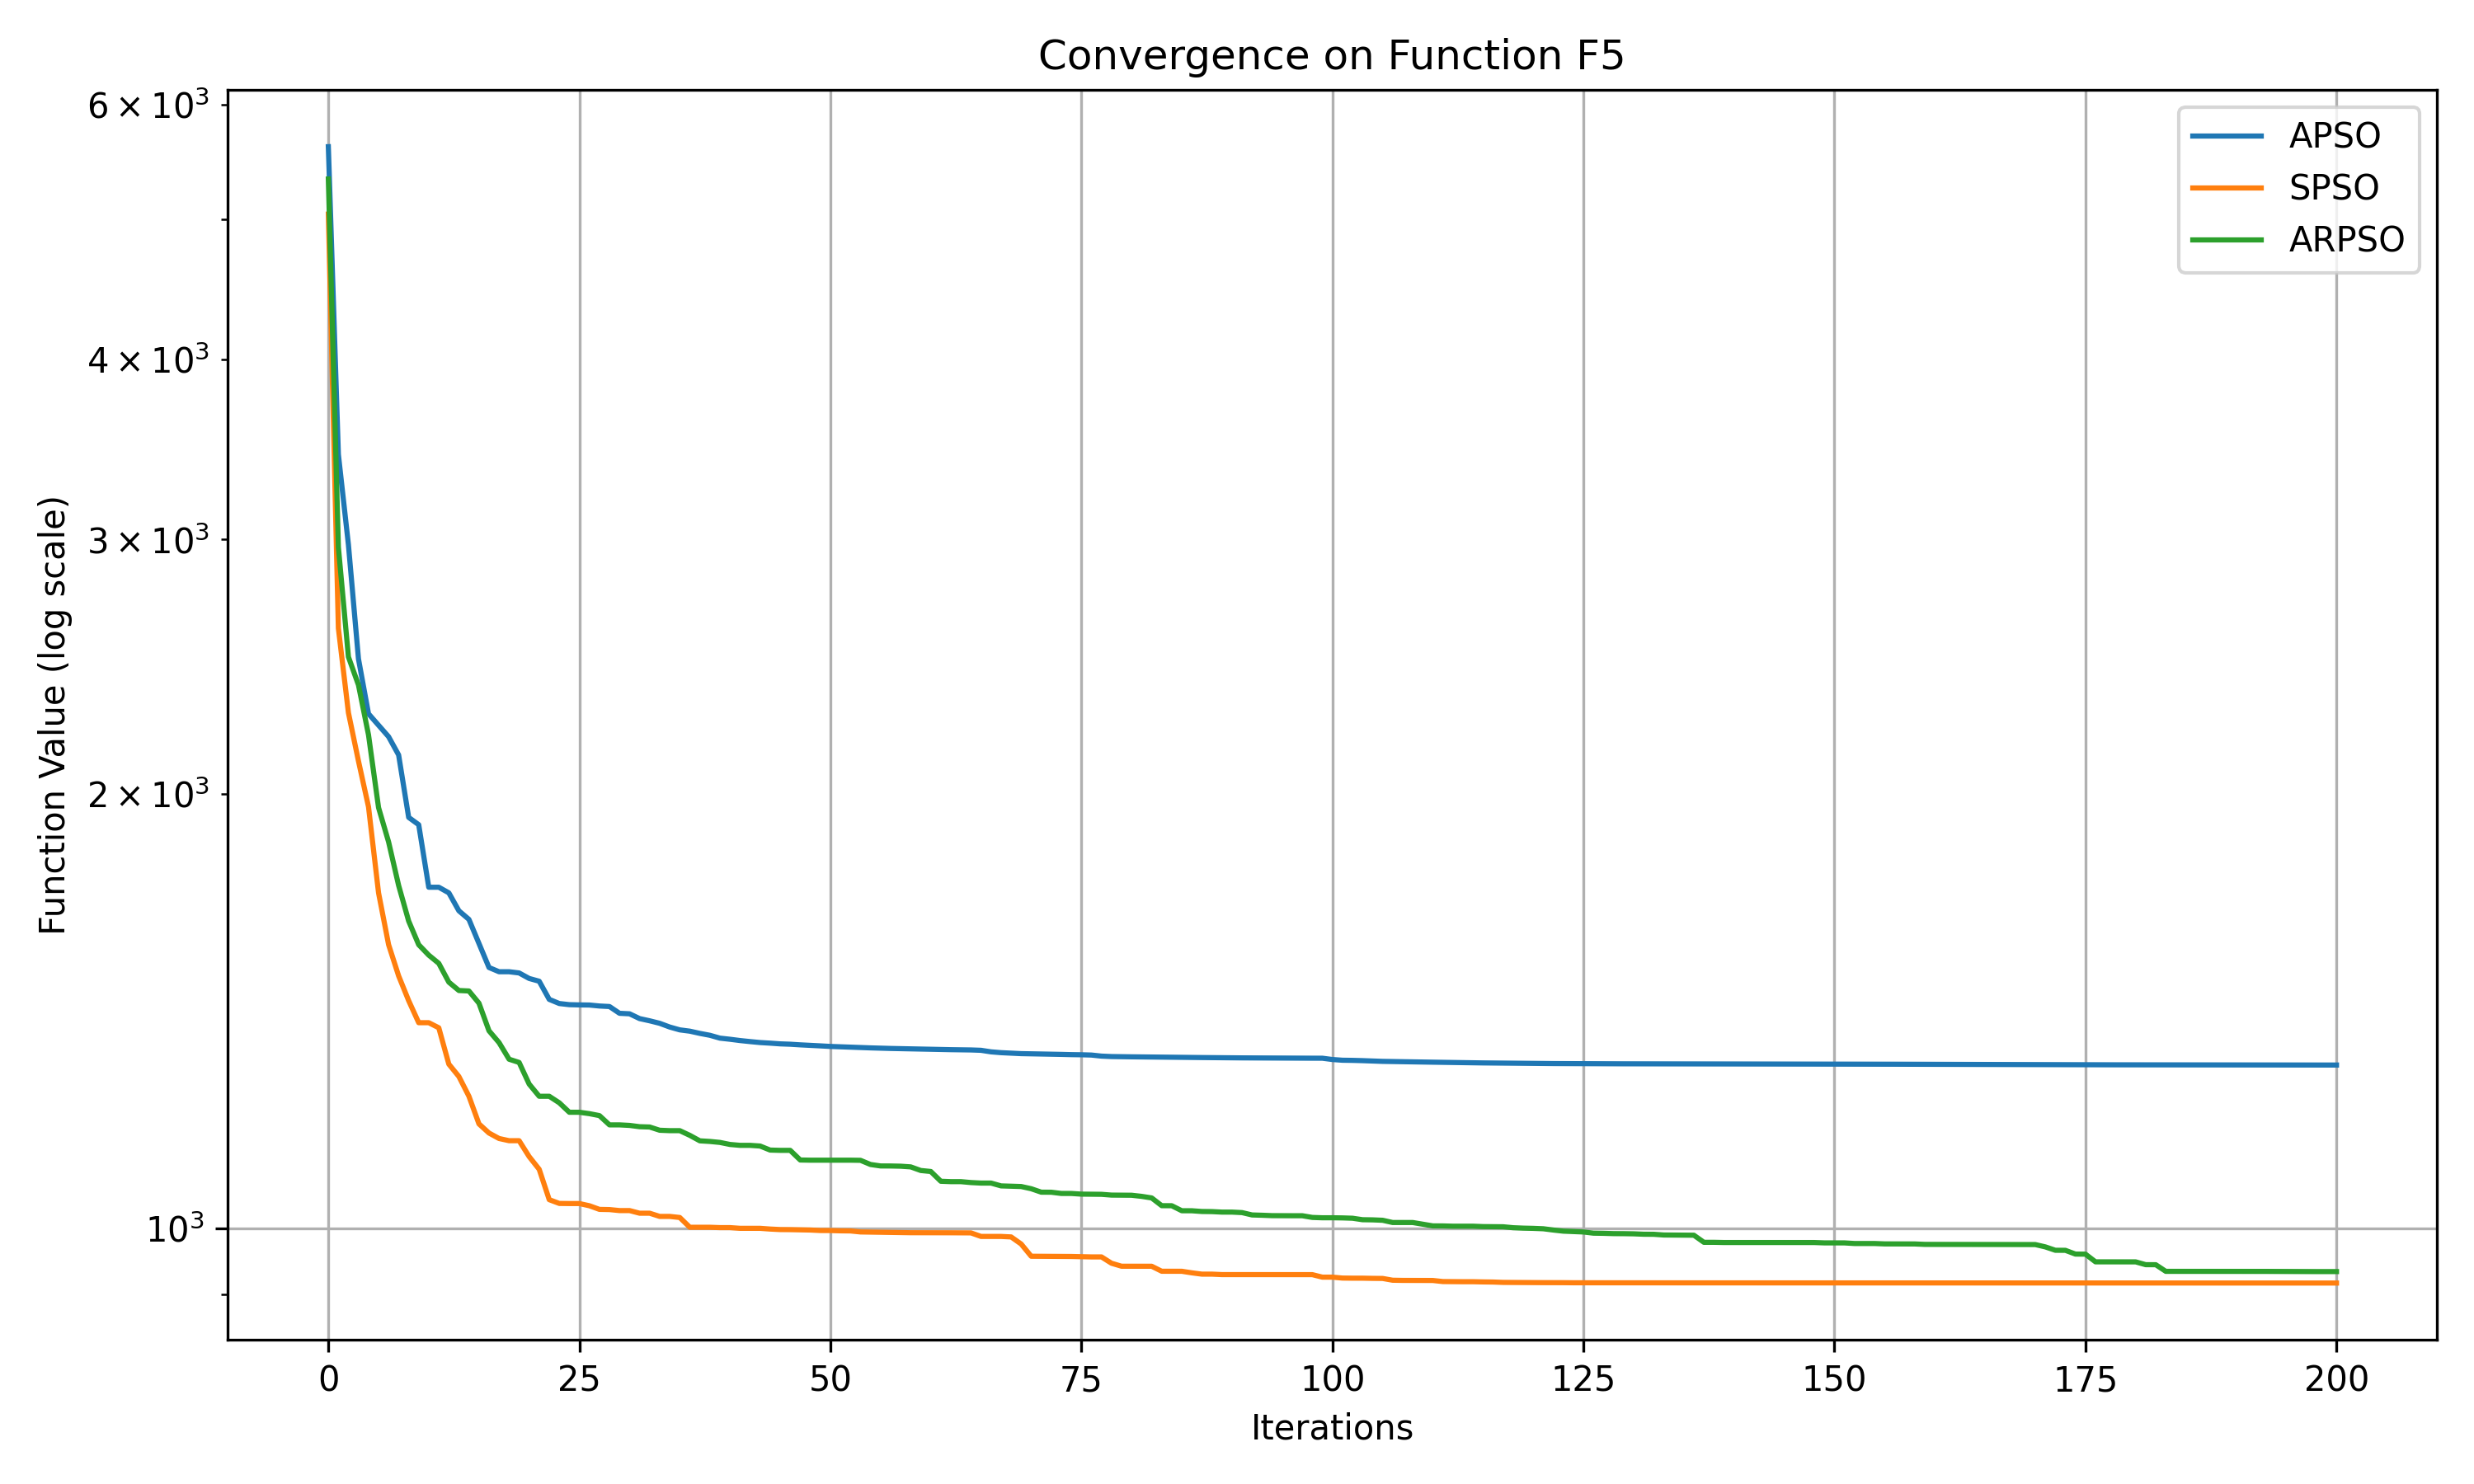
\includegraphics[width=\textwidth]{../plots/cec_bench/cec_convergence_f5.png}
            \caption*{F5 convergence}
        \end{subfigure}
        \vspace{-1ex}
        \caption*{\scriptsize Convergence Plots}
    \end{figure}
\end{frame}

\begin{frame}{Observations}
    \begin{itemize}
        \item \textbf{SPSO performs best overall:} The radar chart and numerical results show SPSO generally finding better solutions (lower values) across most functions, particularly on F1, F3, F4, and F5.
        \item \textbf{APSO shows mixed performance:} It performs well on some functions (F2, F4) but struggles with others (F1, F5), showing higher variability (larger standard deviations).
        \item \textbf{ARPSO consistently underperforms:} It generally finds worse solutions than the other algorithms, especially on F3 and F4, which matches its design as prioritizing exploration over exploitation.
    \end{itemize}
\end{frame}
\begin{frame}{Continued}
    \begin{itemize}
        \item \textbf{F1 (Zakharov Function)}
        \begin{itemize}
            \item SPSO performs best, APSO shows high variability
            \item The convergence plot shows SPSO eventually finding better solutions after 150+ iterations
            \item \textbf{Zakharov relatively smooth but has interdependent variables. APSO's momentum can sometimes overshoot, explaining its variability, while SPSO's balanced approach works well.}
        \end{itemize}
        \item \textbf{APSO:} faster initial convergence (F2, F4) but plateaus earlier. This matches its acceleration based design , momentum helps it make quick progress but make fine adjustments difficult.
        \item \textbf{SPSO:} steady, consistent improvement and achieves the best final solutions (F1, F3, F5). Its balanced approach allows it to both explore broadly and refine solutions effectively.
        \item \textbf{ARPSO:} plateaus early (F3, F4) but occasionally shows late improvements (F1). The added randomness helps it escape local optima but can prevent focused exploitation.
    \end{itemize}
\end{frame}

% % % % ------------------------ Refrence ------------------------
\begin{frame}{References}
    \bibliographystyle{plain}
    \bibliography{refrence}    
\end{frame}
\end{document}